\documentclass[twoside]{book}

% Packages required by doxygen
\usepackage{fixltx2e}
\usepackage{calc}
\usepackage{doxygen}
\usepackage[export]{adjustbox} % also loads graphicx
\usepackage{graphicx}
\usepackage[utf8]{inputenc}
\usepackage{makeidx}
\usepackage{multicol}
\usepackage{multirow}
\PassOptionsToPackage{warn}{textcomp}
\usepackage{textcomp}
\usepackage[nointegrals]{wasysym}
\usepackage[table]{xcolor}

% Font selection
\usepackage[T1]{fontenc}
\usepackage[scaled=.90]{helvet}
\usepackage{courier}
\usepackage{amssymb}
\usepackage{sectsty}
\renewcommand{\familydefault}{\sfdefault}
\allsectionsfont{%
  \fontseries{bc}\selectfont%
  \color{darkgray}%
}
\renewcommand{\DoxyLabelFont}{%
  \fontseries{bc}\selectfont%
  \color{darkgray}%
}
\newcommand{\+}{\discretionary{\mbox{\scriptsize$\hookleftarrow$}}{}{}}

% Page & text layout
\usepackage{geometry}
\geometry{%
  a4paper,%
  top=2.5cm,%
  bottom=2.5cm,%
  left=2.5cm,%
  right=2.5cm%
}
\tolerance=750
\hfuzz=15pt
\hbadness=750
\setlength{\emergencystretch}{15pt}
\setlength{\parindent}{0cm}
\setlength{\parskip}{3ex plus 2ex minus 2ex}
\makeatletter
\renewcommand{\paragraph}{%
  \@startsection{paragraph}{4}{0ex}{-1.0ex}{1.0ex}{%
    \normalfont\normalsize\bfseries\SS@parafont%
  }%
}
\renewcommand{\subparagraph}{%
  \@startsection{subparagraph}{5}{0ex}{-1.0ex}{1.0ex}{%
    \normalfont\normalsize\bfseries\SS@subparafont%
  }%
}
\makeatother

% Headers & footers
\usepackage{fancyhdr}
\pagestyle{fancyplain}
\fancyhead[LE]{\fancyplain{}{\bfseries\thepage}}
\fancyhead[CE]{\fancyplain{}{}}
\fancyhead[RE]{\fancyplain{}{\bfseries\leftmark}}
\fancyhead[LO]{\fancyplain{}{\bfseries\rightmark}}
\fancyhead[CO]{\fancyplain{}{}}
\fancyhead[RO]{\fancyplain{}{\bfseries\thepage}}
\fancyfoot[LE]{\fancyplain{}{}}
\fancyfoot[CE]{\fancyplain{}{}}
\fancyfoot[RE]{\fancyplain{}{\bfseries\scriptsize Generated by Doxygen }}
\fancyfoot[LO]{\fancyplain{}{\bfseries\scriptsize Generated by Doxygen }}
\fancyfoot[CO]{\fancyplain{}{}}
\fancyfoot[RO]{\fancyplain{}{}}
\renewcommand{\footrulewidth}{0.4pt}
\renewcommand{\chaptermark}[1]{%
  \markboth{#1}{}%
}
\renewcommand{\sectionmark}[1]{%
  \markright{\thesection\ #1}%
}

% Indices & bibliography
\usepackage{natbib}
\usepackage[titles]{tocloft}
\setcounter{tocdepth}{3}
\setcounter{secnumdepth}{5}
\makeindex

% Hyperlinks (required, but should be loaded last)
\usepackage{ifpdf}
\ifpdf
  \usepackage[pdftex,pagebackref=true]{hyperref}
\else
  \usepackage[ps2pdf,pagebackref=true]{hyperref}
\fi
\hypersetup{%
  colorlinks=true,%
  linkcolor=blue,%
  citecolor=blue,%
  unicode%
}

% Custom commands
\newcommand{\clearemptydoublepage}{%
  \newpage{\pagestyle{empty}\cleardoublepage}%
}

\usepackage{caption}
\captionsetup{labelsep=space,justification=centering,font={bf},singlelinecheck=off,skip=4pt,position=top}

%===== C O N T E N T S =====

\begin{document}

% Titlepage & ToC
\hypersetup{pageanchor=false,
             bookmarksnumbered=true,
             pdfencoding=unicode
            }
\pagenumbering{roman}
\begin{titlepage}
\vspace*{7cm}
\begin{center}%
{\Large My Project }\\
\vspace*{1cm}
{\large Generated by Doxygen 1.8.11}\\
\end{center}
\end{titlepage}
\clearemptydoublepage
\tableofcontents
\clearemptydoublepage
\pagenumbering{arabic}
\hypersetup{pageanchor=true}

%--- Begin generated contents ---
\chapter{Hierarchical Index}
\section{Class Hierarchy}
This inheritance list is sorted roughly, but not completely, alphabetically\+:\begin{DoxyCompactList}
\item \contentsline{section}{Check\+Clave}{\pageref{class_check_clave}}{}
\item exception\begin{DoxyCompactList}
\item \contentsline{section}{existing\+\_\+user}{\pageref{classexisting__user}}{}
\item \contentsline{section}{file\+\_\+not\+\_\+found}{\pageref{classfile__not__found}}{}
\item \contentsline{section}{password\+\_\+not\+\_\+accepted}{\pageref{classpassword__not__accepted}}{}
\item \contentsline{section}{user\+\_\+not\+\_\+found}{\pageref{classuser__not__found}}{}
\end{DoxyCompactList}
\item \contentsline{section}{Gestor\+Usuarios}{\pageref{class_gestor_usuarios}}{}
\item \contentsline{section}{Usuario}{\pageref{class_usuario}}{}
\end{DoxyCompactList}

\chapter{Class Index}
\section{Class List}
Here are the classes, structs, unions and interfaces with brief descriptions\+:\begin{DoxyCompactList}
\item\contentsline{section}{\hyperlink{class_check_clave}{Check\+Clave} }{\pageref{class_check_clave}}{}
\item\contentsline{section}{\hyperlink{classexisting__user}{existing\+\_\+user} }{\pageref{classexisting__user}}{}
\item\contentsline{section}{\hyperlink{classfile__not__found}{file\+\_\+not\+\_\+found} }{\pageref{classfile__not__found}}{}
\item\contentsline{section}{\hyperlink{class_gestor_usuarios}{Gestor\+Usuarios} }{\pageref{class_gestor_usuarios}}{}
\item\contentsline{section}{\hyperlink{classpassword__not__accepted}{password\+\_\+not\+\_\+accepted} }{\pageref{classpassword__not__accepted}}{}
\item\contentsline{section}{\hyperlink{classuser__not__found}{user\+\_\+not\+\_\+found} }{\pageref{classuser__not__found}}{}
\item\contentsline{section}{\hyperlink{class_usuario}{Usuario} }{\pageref{class_usuario}}{}
\end{DoxyCompactList}

\chapter{File Index}
\section{File List}
Here is a list of all files with brief descriptions\+:\begin{DoxyCompactList}
\item\contentsline{section}{\hyperlink{_check_clave_8cpp}{Check\+Clave.\+cpp} }{\pageref{_check_clave_8cpp}}{}
\item\contentsline{section}{\hyperlink{_check_clave_8h}{Check\+Clave.\+h} }{\pageref{_check_clave_8h}}{}
\item\contentsline{section}{\hyperlink{existing_01user_8h}{existing user.\+h} }{\pageref{existing_01user_8h}}{}
\item\contentsline{section}{\hyperlink{file_01not_01found_8h}{file not found.\+h} }{\pageref{file_01not_01found_8h}}{}
\item\contentsline{section}{\hyperlink{_gestor_usuarios_8cpp}{Gestor\+Usuarios.\+cpp} }{\pageref{_gestor_usuarios_8cpp}}{}
\item\contentsline{section}{\hyperlink{_gestor_usuarios_8h}{Gestor\+Usuarios.\+h} }{\pageref{_gestor_usuarios_8h}}{}
\item\contentsline{section}{\hyperlink{main_8cpp}{main.\+cpp} }{\pageref{main_8cpp}}{}
\item\contentsline{section}{\hyperlink{password_01not_01accepted_8h}{password not accepted.\+h} }{\pageref{password_01not_01accepted_8h}}{}
\item\contentsline{section}{\hyperlink{user_01not_01found_8h}{user not found.\+h} }{\pageref{user_01not_01found_8h}}{}
\item\contentsline{section}{\hyperlink{_usuario_8cpp}{Usuario.\+cpp} }{\pageref{_usuario_8cpp}}{}
\item\contentsline{section}{\hyperlink{_usuario_8h}{Usuario.\+h} }{\pageref{_usuario_8h}}{}
\end{DoxyCompactList}

\chapter{Class Documentation}
\hypertarget{class_check_clave}{}\section{Check\+Clave Class Reference}
\label{class_check_clave}\index{Check\+Clave@{Check\+Clave}}


{\ttfamily \#include $<$Check\+Clave.\+h$>$}

\subsection*{Public Member Functions}
\begin{DoxyCompactItemize}
\item 
\hyperlink{class_check_clave_a33e8b9961db4afa6559433f0c6b40473}{Check\+Clave} ()
\item 
\hyperlink{class_check_clave_a3d2a6a9d993f6fca98c5179a34dc8aad}{Check\+Clave} (\hyperlink{class_check_clave}{Check\+Clave} \&orig)
\item 
virtual \hyperlink{class_check_clave_a5806c7ceb4604ee952f4f42f12a55994}{$\sim$\+Check\+Clave} ()
\item 
\hyperlink{class_check_clave}{Check\+Clave} \& \hyperlink{class_check_clave_a08b17f5832d841c1dbe09c92ec542b47}{operator=} (\hyperlink{class_check_clave}{Check\+Clave} \&c)
\item 
int \hyperlink{class_check_clave_a7f2bf7386f3f4d3ae9bc0811141fcaa2}{check} (string \&s)
\end{DoxyCompactItemize}


\subsection{Detailed Description}
Check\+Key class 

Definition at line 19 of file Check\+Clave.\+h.



\subsection{Constructor \& Destructor Documentation}
\index{Check\+Clave@{Check\+Clave}!Check\+Clave@{Check\+Clave}}
\index{Check\+Clave@{Check\+Clave}!Check\+Clave@{Check\+Clave}}
\subsubsection[{\texorpdfstring{Check\+Clave()}{CheckClave()}}]{\setlength{\rightskip}{0pt plus 5cm}Check\+Clave\+::\+Check\+Clave (
\begin{DoxyParamCaption}
{}
\end{DoxyParamCaption}
)}\hypertarget{class_check_clave_a33e8b9961db4afa6559433f0c6b40473}{}\label{class_check_clave_a33e8b9961db4afa6559433f0c6b40473}
Check\+Key constructor read the file lemario-\/espanol-\/utf8.\+txt and initialize tree 

Definition at line 16 of file Check\+Clave.\+cpp.

\index{Check\+Clave@{Check\+Clave}!Check\+Clave@{Check\+Clave}}
\index{Check\+Clave@{Check\+Clave}!Check\+Clave@{Check\+Clave}}
\subsubsection[{\texorpdfstring{Check\+Clave(\+Check\+Clave \&orig)}{CheckClave(CheckClave &orig)}}]{\setlength{\rightskip}{0pt plus 5cm}Check\+Clave\+::\+Check\+Clave (
\begin{DoxyParamCaption}
\item[{{\bf Check\+Clave} \&}]{orig}
\end{DoxyParamCaption}
)}\hypertarget{class_check_clave_a3d2a6a9d993f6fca98c5179a34dc8aad}{}\label{class_check_clave_a3d2a6a9d993f6fca98c5179a34dc8aad}
Check\+Key copy constructor 
\begin{DoxyParams}{Parameters}
{\em orig} & a check\+Key \\
\hline
\end{DoxyParams}


Definition at line 35 of file Check\+Clave.\+cpp.

\index{Check\+Clave@{Check\+Clave}!````~Check\+Clave@{$\sim$\+Check\+Clave}}
\index{````~Check\+Clave@{$\sim$\+Check\+Clave}!Check\+Clave@{Check\+Clave}}
\subsubsection[{\texorpdfstring{$\sim$\+Check\+Clave()}{~CheckClave()}}]{\setlength{\rightskip}{0pt plus 5cm}Check\+Clave\+::$\sim$\+Check\+Clave (
\begin{DoxyParamCaption}
{}
\end{DoxyParamCaption}
)\hspace{0.3cm}{\ttfamily [virtual]}}\hypertarget{class_check_clave_a5806c7ceb4604ee952f4f42f12a55994}{}\label{class_check_clave_a5806c7ceb4604ee952f4f42f12a55994}
Check\+Key destructor 

Definition at line 41 of file Check\+Clave.\+cpp.



\subsection{Member Function Documentation}
\index{Check\+Clave@{Check\+Clave}!check@{check}}
\index{check@{check}!Check\+Clave@{Check\+Clave}}
\subsubsection[{\texorpdfstring{check(string \&s)}{check(string &s)}}]{\setlength{\rightskip}{0pt plus 5cm}int Check\+Clave\+::check (
\begin{DoxyParamCaption}
\item[{string \&}]{s}
\end{DoxyParamCaption}
)}\hypertarget{class_check_clave_a7f2bf7386f3f4d3ae9bc0811141fcaa2}{}\label{class_check_clave_a7f2bf7386f3f4d3ae9bc0811141fcaa2}
Check function check is the password is correct, if it is correct return 0 
\begin{DoxyParams}{Parameters}
{\em s} & a word \\
\hline
\end{DoxyParams}
\begin{DoxyReturn}{Returns}
an integer (0 if key is correct) 
\end{DoxyReturn}


Definition at line 60 of file Check\+Clave.\+cpp.



Here is the caller graph for this function\+:\nopagebreak
\begin{figure}[H]
\begin{center}
\leavevmode
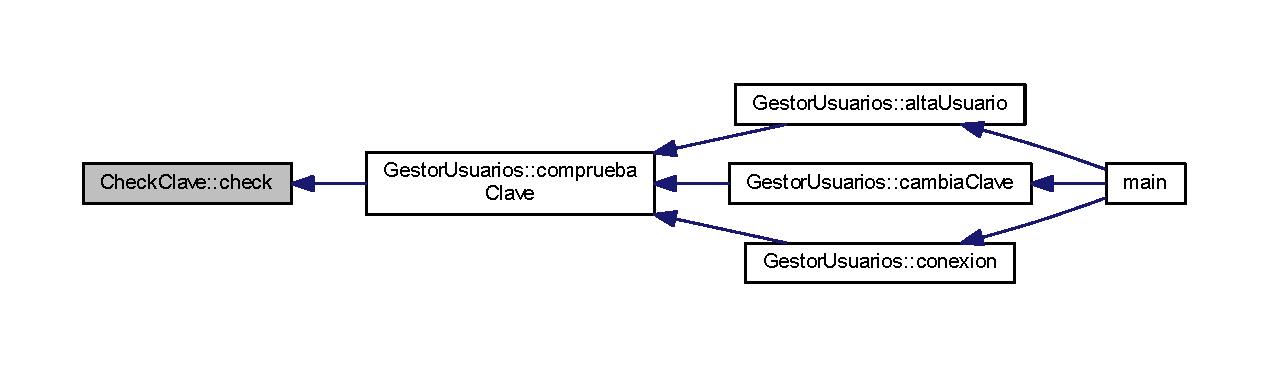
\includegraphics[width=350pt]{class_check_clave_a7f2bf7386f3f4d3ae9bc0811141fcaa2_icgraph}
\end{center}
\end{figure}


\index{Check\+Clave@{Check\+Clave}!operator=@{operator=}}
\index{operator=@{operator=}!Check\+Clave@{Check\+Clave}}
\subsubsection[{\texorpdfstring{operator=(\+Check\+Clave \&c)}{operator=(CheckClave &c)}}]{\setlength{\rightskip}{0pt plus 5cm}{\bf Check\+Clave} \& Check\+Clave\+::operator= (
\begin{DoxyParamCaption}
\item[{{\bf Check\+Clave} \&}]{c}
\end{DoxyParamCaption}
)}\hypertarget{class_check_clave_a08b17f5832d841c1dbe09c92ec542b47}{}\label{class_check_clave_a08b17f5832d841c1dbe09c92ec542b47}
Operator= Check\+Key define operator = 
\begin{DoxyParams}{Parameters}
{\em c} & a check\+Key \\
\hline
\end{DoxyParams}
\begin{DoxyReturn}{Returns}
a check\+Key 
\end{DoxyReturn}


Definition at line 50 of file Check\+Clave.\+cpp.



The documentation for this class was generated from the following files\+:\begin{DoxyCompactItemize}
\item 
\hyperlink{_check_clave_8h}{Check\+Clave.\+h}\item 
\hyperlink{_check_clave_8cpp}{Check\+Clave.\+cpp}\end{DoxyCompactItemize}

\hypertarget{classexisting__user}{}\section{existing\+\_\+user Class Reference}
\label{classexisting__user}\index{existing\+\_\+user@{existing\+\_\+user}}


{\ttfamily \#include $<$existing user.\+h$>$}



Inheritance diagram for existing\+\_\+user\+:\nopagebreak
\begin{figure}[H]
\begin{center}
\leavevmode
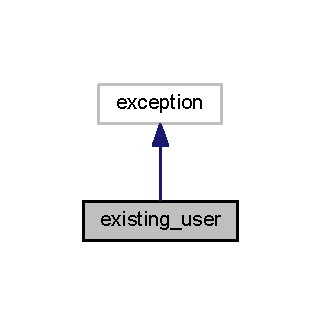
\includegraphics[width=154pt]{classexisting__user__inherit__graph}
\end{center}
\end{figure}


Collaboration diagram for existing\+\_\+user\+:\nopagebreak
\begin{figure}[H]
\begin{center}
\leavevmode
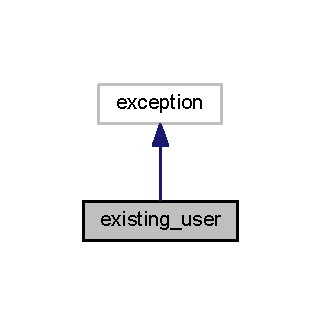
\includegraphics[width=154pt]{classexisting__user__coll__graph}
\end{center}
\end{figure}
\subsection*{Public Member Functions}
\begin{DoxyCompactItemize}
\item 
virtual const char $\ast$ \hyperlink{classexisting__user_a2df7d83617d1c130f36887f5b765760e}{what} () const   throw ()
\item 
virtual \hyperlink{classexisting__user_a1abb8f60e30bb9932f003c64d6d90f59}{$\sim$existing\+\_\+user} ()  throw ()
\end{DoxyCompactItemize}


\subsection{Detailed Description}
Existing user exception 

Definition at line 15 of file existing user.\+h.



\subsection{Constructor \& Destructor Documentation}
\index{existing\+\_\+user@{existing\+\_\+user}!````~existing\+\_\+user@{$\sim$existing\+\_\+user}}
\index{````~existing\+\_\+user@{$\sim$existing\+\_\+user}!existing\+\_\+user@{existing\+\_\+user}}
\subsubsection[{\texorpdfstring{$\sim$existing\+\_\+user()}{~existing_user()}}]{\setlength{\rightskip}{0pt plus 5cm}virtual existing\+\_\+user\+::$\sim$existing\+\_\+user (
\begin{DoxyParamCaption}
{}
\end{DoxyParamCaption}
) throw  ) \hspace{0.3cm}{\ttfamily [inline]}, {\ttfamily [virtual]}}\hypertarget{classexisting__user_a1abb8f60e30bb9932f003c64d6d90f59}{}\label{classexisting__user_a1abb8f60e30bb9932f003c64d6d90f59}


Definition at line 25 of file existing user.\+h.



\subsection{Member Function Documentation}
\index{existing\+\_\+user@{existing\+\_\+user}!what@{what}}
\index{what@{what}!existing\+\_\+user@{existing\+\_\+user}}
\subsubsection[{\texorpdfstring{what() const }{what() const }}]{\setlength{\rightskip}{0pt plus 5cm}virtual const char$\ast$ existing\+\_\+user\+::what (
\begin{DoxyParamCaption}
{}
\end{DoxyParamCaption}
) const throw  ) \hspace{0.3cm}{\ttfamily [inline]}, {\ttfamily [virtual]}}\hypertarget{classexisting__user_a2df7d83617d1c130f36887f5b765760e}{}\label{classexisting__user_a2df7d83617d1c130f36887f5b765760e}
A exception Show the exception when user already exists in the system \begin{DoxyReturn}{Returns}

\end{DoxyReturn}


Definition at line 22 of file existing user.\+h.



The documentation for this class was generated from the following file\+:\begin{DoxyCompactItemize}
\item 
\hyperlink{existing_01user_8h}{existing user.\+h}\end{DoxyCompactItemize}

\hypertarget{classfile__not__found}{}\section{file\+\_\+not\+\_\+found Class Reference}
\label{classfile__not__found}\index{file\+\_\+not\+\_\+found@{file\+\_\+not\+\_\+found}}


{\ttfamily \#include $<$file not found.\+h$>$}



Inheritance diagram for file\+\_\+not\+\_\+found\+:\nopagebreak
\begin{figure}[H]
\begin{center}
\leavevmode
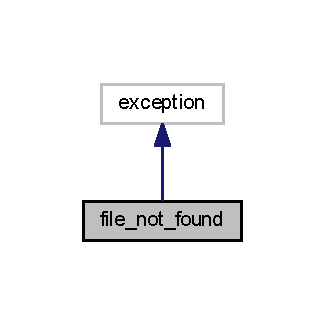
\includegraphics[width=156pt]{classfile__not__found__inherit__graph}
\end{center}
\end{figure}


Collaboration diagram for file\+\_\+not\+\_\+found\+:\nopagebreak
\begin{figure}[H]
\begin{center}
\leavevmode
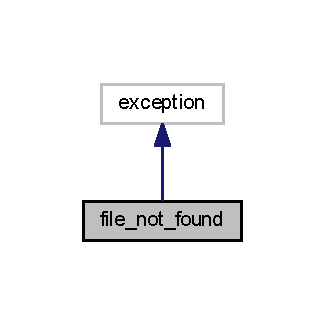
\includegraphics[width=156pt]{classfile__not__found__coll__graph}
\end{center}
\end{figure}
\subsection*{Public Member Functions}
\begin{DoxyCompactItemize}
\item 
virtual const char $\ast$ \hyperlink{classfile__not__found_a082aafca4de0a7ea87aa45dc2a85cddf}{what} () const   throw ()
\item 
virtual \hyperlink{classfile__not__found_a533bcc14073a910ec2193c31357c96a9}{$\sim$file\+\_\+not\+\_\+found} ()  throw ()
\end{DoxyCompactItemize}


\subsection{Detailed Description}
File not found exception 

Definition at line 15 of file file not found.\+h.



\subsection{Constructor \& Destructor Documentation}
\index{file\+\_\+not\+\_\+found@{file\+\_\+not\+\_\+found}!````~file\+\_\+not\+\_\+found@{$\sim$file\+\_\+not\+\_\+found}}
\index{````~file\+\_\+not\+\_\+found@{$\sim$file\+\_\+not\+\_\+found}!file\+\_\+not\+\_\+found@{file\+\_\+not\+\_\+found}}
\subsubsection[{\texorpdfstring{$\sim$file\+\_\+not\+\_\+found()}{~file_not_found()}}]{\setlength{\rightskip}{0pt plus 5cm}virtual file\+\_\+not\+\_\+found\+::$\sim$file\+\_\+not\+\_\+found (
\begin{DoxyParamCaption}
{}
\end{DoxyParamCaption}
) throw  ) \hspace{0.3cm}{\ttfamily [inline]}, {\ttfamily [virtual]}}\hypertarget{classfile__not__found_a533bcc14073a910ec2193c31357c96a9}{}\label{classfile__not__found_a533bcc14073a910ec2193c31357c96a9}


Definition at line 25 of file file not found.\+h.



\subsection{Member Function Documentation}
\index{file\+\_\+not\+\_\+found@{file\+\_\+not\+\_\+found}!what@{what}}
\index{what@{what}!file\+\_\+not\+\_\+found@{file\+\_\+not\+\_\+found}}
\subsubsection[{\texorpdfstring{what() const }{what() const }}]{\setlength{\rightskip}{0pt plus 5cm}virtual const char$\ast$ file\+\_\+not\+\_\+found\+::what (
\begin{DoxyParamCaption}
{}
\end{DoxyParamCaption}
) const throw  ) \hspace{0.3cm}{\ttfamily [inline]}, {\ttfamily [virtual]}}\hypertarget{classfile__not__found_a082aafca4de0a7ea87aa45dc2a85cddf}{}\label{classfile__not__found_a082aafca4de0a7ea87aa45dc2a85cddf}
A exception Show the exception when the file is not found \begin{DoxyReturn}{Returns}

\end{DoxyReturn}


Definition at line 22 of file file not found.\+h.



The documentation for this class was generated from the following file\+:\begin{DoxyCompactItemize}
\item 
\hyperlink{file_01not_01found_8h}{file not found.\+h}\end{DoxyCompactItemize}

\hypertarget{class_gestor_usuarios}{}\section{Gestor\+Usuarios Class Reference}
\label{class_gestor_usuarios}\index{Gestor\+Usuarios@{Gestor\+Usuarios}}


{\ttfamily \#include $<$Gestor\+Usuarios.\+h$>$}

\subsection*{Public Member Functions}
\begin{DoxyCompactItemize}
\item 
\hyperlink{class_gestor_usuarios_a5e10ca400b0d699a70aa9aba8189b389}{Gestor\+Usuarios} ()
\item 
\hyperlink{class_gestor_usuarios_a540f562d1cc4e775874ca59fb58460f2}{Gestor\+Usuarios} (\hyperlink{class_gestor_usuarios}{Gestor\+Usuarios} \&orig)
\item 
virtual \hyperlink{class_gestor_usuarios_a5d3e11b3129b1d988fe045cf38518ccb}{$\sim$\+Gestor\+Usuarios} ()
\item 
\hyperlink{class_gestor_usuarios}{Gestor\+Usuarios} \& \hyperlink{class_gestor_usuarios_abd8499f2178dc4e730674a78ecddae79}{operator=} (\hyperlink{class_gestor_usuarios}{Gestor\+Usuarios} \&g)
\item 
void \hyperlink{class_gestor_usuarios_a0c04ca0167fd1f00d8df198441763311}{alta\+Usuario} (\hyperlink{class_usuario}{Usuario} \&u)
\item 
void \hyperlink{class_gestor_usuarios_a68d73f9a0ede622220012502ffc23dcf}{baja\+Usuario} (string \&id)
\item 
void \hyperlink{class_gestor_usuarios_ad14240167762426efe2c8f2af2421fe0}{cambia\+Clave} (string \&id, string \&clave)
\item 
\hyperlink{class_usuario}{Usuario} \& \hyperlink{class_gestor_usuarios_a7f941f9780501cd260591a96ba30d048}{busca\+Usuario} (string \&id)
\item 
void \hyperlink{class_gestor_usuarios_a3b929870c33c4864d3c1f32f2614a64d}{conexion} (string \&id, string \&clave)
\item 
void \hyperlink{class_gestor_usuarios_a1e57859037abf37a190ad2c60ed22f2b}{desconexion} (string \&id)
\item 
bool \hyperlink{class_gestor_usuarios_a41196c2a9b3abd71e7eb8f79fd765960}{esta\+Conectado} (string \&id)
\item 
set$<$ string $>$ \hyperlink{class_gestor_usuarios_a2a20b4c548e4bbe113174a416873194a}{usuarios\+Conectados} ()
\item 
bool \hyperlink{class_gestor_usuarios_a14c8dfce3dabbbdc4cd6214e6093ed60}{comprueba\+Clave} (string \&clave)
\end{DoxyCompactItemize}


\subsection{Detailed Description}
Users manager managed users and connect users 

Definition at line 18 of file Gestor\+Usuarios.\+h.



\subsection{Constructor \& Destructor Documentation}
\index{Gestor\+Usuarios@{Gestor\+Usuarios}!Gestor\+Usuarios@{Gestor\+Usuarios}}
\index{Gestor\+Usuarios@{Gestor\+Usuarios}!Gestor\+Usuarios@{Gestor\+Usuarios}}
\subsubsection[{\texorpdfstring{Gestor\+Usuarios()}{GestorUsuarios()}}]{\setlength{\rightskip}{0pt plus 5cm}Gestor\+Usuarios\+::\+Gestor\+Usuarios (
\begin{DoxyParamCaption}
{}
\end{DoxyParamCaption}
)}\hypertarget{class_gestor_usuarios_a5e10ca400b0d699a70aa9aba8189b389}{}\label{class_gestor_usuarios_a5e10ca400b0d699a70aa9aba8189b389}
User manager constructor 

Definition at line 17 of file Gestor\+Usuarios.\+cpp.

\index{Gestor\+Usuarios@{Gestor\+Usuarios}!Gestor\+Usuarios@{Gestor\+Usuarios}}
\index{Gestor\+Usuarios@{Gestor\+Usuarios}!Gestor\+Usuarios@{Gestor\+Usuarios}}
\subsubsection[{\texorpdfstring{Gestor\+Usuarios(\+Gestor\+Usuarios \&orig)}{GestorUsuarios(GestorUsuarios &orig)}}]{\setlength{\rightskip}{0pt plus 5cm}Gestor\+Usuarios\+::\+Gestor\+Usuarios (
\begin{DoxyParamCaption}
\item[{{\bf Gestor\+Usuarios} \&}]{orig}
\end{DoxyParamCaption}
)}\hypertarget{class_gestor_usuarios_a540f562d1cc4e775874ca59fb58460f2}{}\label{class_gestor_usuarios_a540f562d1cc4e775874ca59fb58460f2}
User manager copy constructor 
\begin{DoxyParams}{Parameters}
{\em orig} & \\
\hline
\end{DoxyParams}


Definition at line 23 of file Gestor\+Usuarios.\+cpp.



Here is the call graph for this function\+:\nopagebreak
\begin{figure}[H]
\begin{center}
\leavevmode
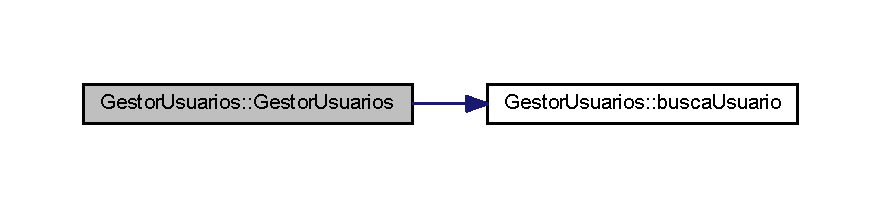
\includegraphics[width=350pt]{class_gestor_usuarios_a540f562d1cc4e775874ca59fb58460f2_cgraph}
\end{center}
\end{figure}


\index{Gestor\+Usuarios@{Gestor\+Usuarios}!````~Gestor\+Usuarios@{$\sim$\+Gestor\+Usuarios}}
\index{````~Gestor\+Usuarios@{$\sim$\+Gestor\+Usuarios}!Gestor\+Usuarios@{Gestor\+Usuarios}}
\subsubsection[{\texorpdfstring{$\sim$\+Gestor\+Usuarios()}{~GestorUsuarios()}}]{\setlength{\rightskip}{0pt plus 5cm}Gestor\+Usuarios\+::$\sim$\+Gestor\+Usuarios (
\begin{DoxyParamCaption}
{}
\end{DoxyParamCaption}
)\hspace{0.3cm}{\ttfamily [virtual]}}\hypertarget{class_gestor_usuarios_a5d3e11b3129b1d988fe045cf38518ccb}{}\label{class_gestor_usuarios_a5d3e11b3129b1d988fe045cf38518ccb}
User manager destructor 

Definition at line 39 of file Gestor\+Usuarios.\+cpp.



\subsection{Member Function Documentation}
\index{Gestor\+Usuarios@{Gestor\+Usuarios}!alta\+Usuario@{alta\+Usuario}}
\index{alta\+Usuario@{alta\+Usuario}!Gestor\+Usuarios@{Gestor\+Usuarios}}
\subsubsection[{\texorpdfstring{alta\+Usuario(\+Usuario \&u)}{altaUsuario(Usuario &u)}}]{\setlength{\rightskip}{0pt plus 5cm}void Gestor\+Usuarios\+::alta\+Usuario (
\begin{DoxyParamCaption}
\item[{{\bf Usuario} \&}]{u}
\end{DoxyParamCaption}
)}\hypertarget{class_gestor_usuarios_a0c04ca0167fd1f00d8df198441763311}{}\label{class_gestor_usuarios_a0c04ca0167fd1f00d8df198441763311}
To register user 
\begin{DoxyParams}{Parameters}
{\em u} & user \\
\hline
\end{DoxyParams}


Definition at line 85 of file Gestor\+Usuarios.\+cpp.



Here is the call graph for this function\+:\nopagebreak
\begin{figure}[H]
\begin{center}
\leavevmode
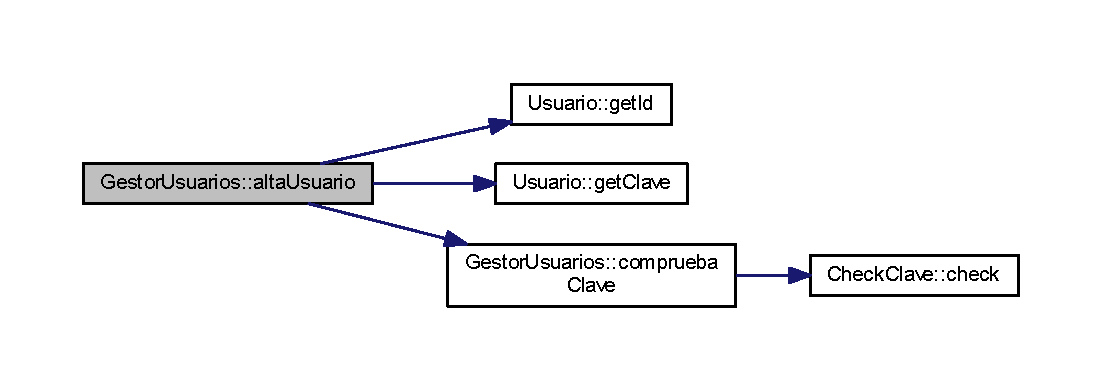
\includegraphics[width=350pt]{class_gestor_usuarios_a0c04ca0167fd1f00d8df198441763311_cgraph}
\end{center}
\end{figure}




Here is the caller graph for this function\+:\nopagebreak
\begin{figure}[H]
\begin{center}
\leavevmode
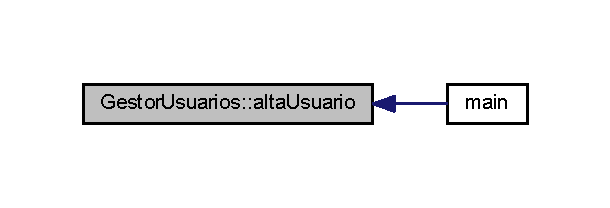
\includegraphics[width=293pt]{class_gestor_usuarios_a0c04ca0167fd1f00d8df198441763311_icgraph}
\end{center}
\end{figure}


\index{Gestor\+Usuarios@{Gestor\+Usuarios}!baja\+Usuario@{baja\+Usuario}}
\index{baja\+Usuario@{baja\+Usuario}!Gestor\+Usuarios@{Gestor\+Usuarios}}
\subsubsection[{\texorpdfstring{baja\+Usuario(string \&id)}{bajaUsuario(string &id)}}]{\setlength{\rightskip}{0pt plus 5cm}void Gestor\+Usuarios\+::baja\+Usuario (
\begin{DoxyParamCaption}
\item[{string \&}]{id}
\end{DoxyParamCaption}
)}\hypertarget{class_gestor_usuarios_a68d73f9a0ede622220012502ffc23dcf}{}\label{class_gestor_usuarios_a68d73f9a0ede622220012502ffc23dcf}
to unsubscribe a user 
\begin{DoxyParams}{Parameters}
{\em id} & of the user \\
\hline
\end{DoxyParams}


Definition at line 103 of file Gestor\+Usuarios.\+cpp.



Here is the call graph for this function\+:\nopagebreak
\begin{figure}[H]
\begin{center}
\leavevmode
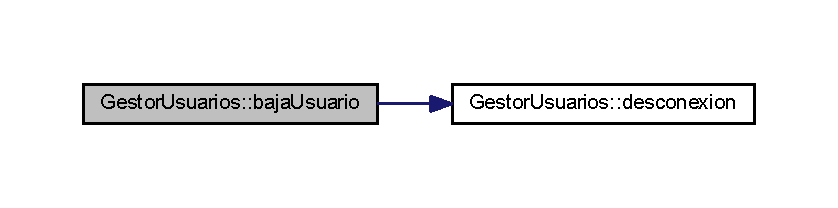
\includegraphics[width=350pt]{class_gestor_usuarios_a68d73f9a0ede622220012502ffc23dcf_cgraph}
\end{center}
\end{figure}




Here is the caller graph for this function\+:\nopagebreak
\begin{figure}[H]
\begin{center}
\leavevmode
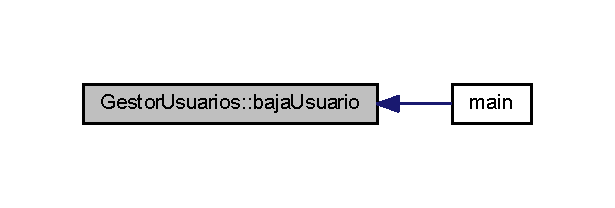
\includegraphics[width=295pt]{class_gestor_usuarios_a68d73f9a0ede622220012502ffc23dcf_icgraph}
\end{center}
\end{figure}


\index{Gestor\+Usuarios@{Gestor\+Usuarios}!busca\+Usuario@{busca\+Usuario}}
\index{busca\+Usuario@{busca\+Usuario}!Gestor\+Usuarios@{Gestor\+Usuarios}}
\subsubsection[{\texorpdfstring{busca\+Usuario(string \&id)}{buscaUsuario(string &id)}}]{\setlength{\rightskip}{0pt plus 5cm}{\bf Usuario} \& Gestor\+Usuarios\+::busca\+Usuario (
\begin{DoxyParamCaption}
\item[{string \&}]{id}
\end{DoxyParamCaption}
)}\hypertarget{class_gestor_usuarios_a7f941f9780501cd260591a96ba30d048}{}\label{class_gestor_usuarios_a7f941f9780501cd260591a96ba30d048}
To find a user 
\begin{DoxyParams}{Parameters}
{\em id} & of the user \\
\hline
\end{DoxyParams}
\begin{DoxyReturn}{Returns}
user found 
\end{DoxyReturn}


Definition at line 143 of file Gestor\+Usuarios.\+cpp.



Here is the caller graph for this function\+:\nopagebreak
\begin{figure}[H]
\begin{center}
\leavevmode
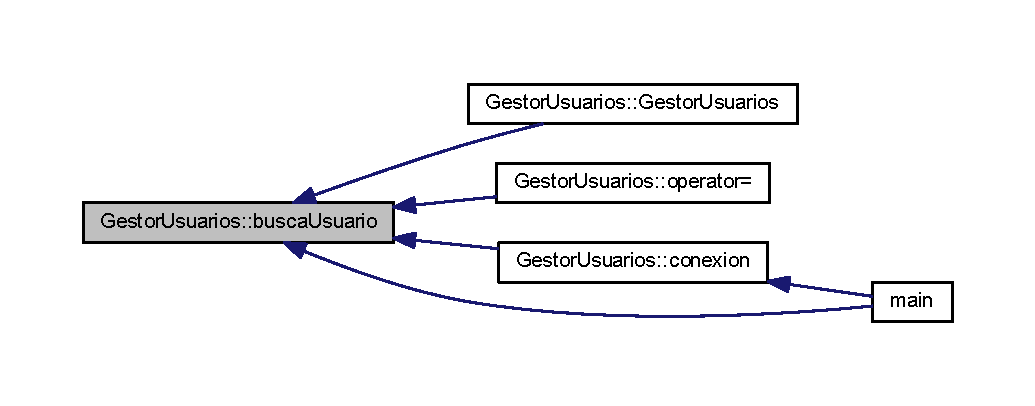
\includegraphics[width=350pt]{class_gestor_usuarios_a7f941f9780501cd260591a96ba30d048_icgraph}
\end{center}
\end{figure}


\index{Gestor\+Usuarios@{Gestor\+Usuarios}!cambia\+Clave@{cambia\+Clave}}
\index{cambia\+Clave@{cambia\+Clave}!Gestor\+Usuarios@{Gestor\+Usuarios}}
\subsubsection[{\texorpdfstring{cambia\+Clave(string \&id, string \&clave)}{cambiaClave(string &id, string &clave)}}]{\setlength{\rightskip}{0pt plus 5cm}void Gestor\+Usuarios\+::cambia\+Clave (
\begin{DoxyParamCaption}
\item[{string \&}]{id, }
\item[{string \&}]{clave}
\end{DoxyParamCaption}
)}\hypertarget{class_gestor_usuarios_ad14240167762426efe2c8f2af2421fe0}{}\label{class_gestor_usuarios_ad14240167762426efe2c8f2af2421fe0}
To change password 
\begin{DoxyParams}{Parameters}
{\em id} & of the user \\
\hline
{\em clave} & key of the user \\
\hline
\end{DoxyParams}


Definition at line 122 of file Gestor\+Usuarios.\+cpp.



Here is the call graph for this function\+:\nopagebreak
\begin{figure}[H]
\begin{center}
\leavevmode
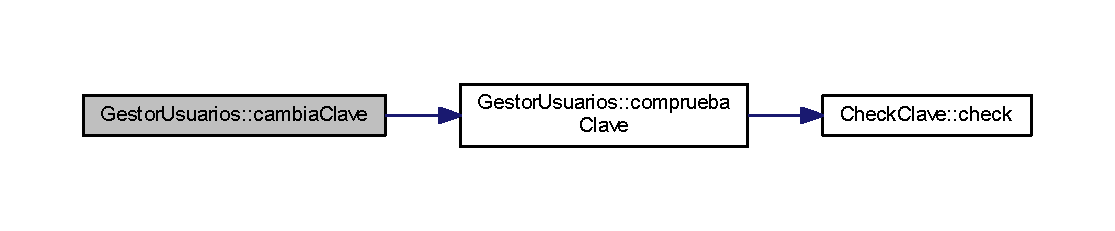
\includegraphics[width=350pt]{class_gestor_usuarios_ad14240167762426efe2c8f2af2421fe0_cgraph}
\end{center}
\end{figure}




Here is the caller graph for this function\+:\nopagebreak
\begin{figure}[H]
\begin{center}
\leavevmode
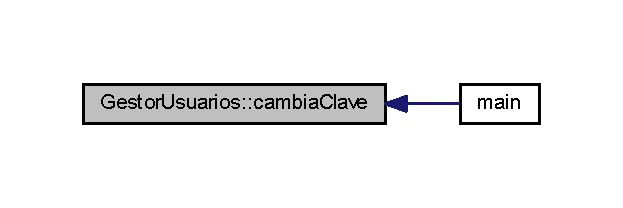
\includegraphics[width=299pt]{class_gestor_usuarios_ad14240167762426efe2c8f2af2421fe0_icgraph}
\end{center}
\end{figure}


\index{Gestor\+Usuarios@{Gestor\+Usuarios}!comprueba\+Clave@{comprueba\+Clave}}
\index{comprueba\+Clave@{comprueba\+Clave}!Gestor\+Usuarios@{Gestor\+Usuarios}}
\subsubsection[{\texorpdfstring{comprueba\+Clave(string \&clave)}{compruebaClave(string &clave)}}]{\setlength{\rightskip}{0pt plus 5cm}bool Gestor\+Usuarios\+::comprueba\+Clave (
\begin{DoxyParamCaption}
\item[{string \&}]{clave}
\end{DoxyParamCaption}
)}\hypertarget{class_gestor_usuarios_a14c8dfce3dabbbdc4cd6214e6093ed60}{}\label{class_gestor_usuarios_a14c8dfce3dabbbdc4cd6214e6093ed60}
Check\+Key function check is the key is correct 
\begin{DoxyParams}{Parameters}
{\em clave} & key of user \\
\hline
\end{DoxyParams}
\begin{DoxyReturn}{Returns}
a boolean value 
\end{DoxyReturn}


Definition at line 69 of file Gestor\+Usuarios.\+cpp.



Here is the call graph for this function\+:\nopagebreak
\begin{figure}[H]
\begin{center}
\leavevmode
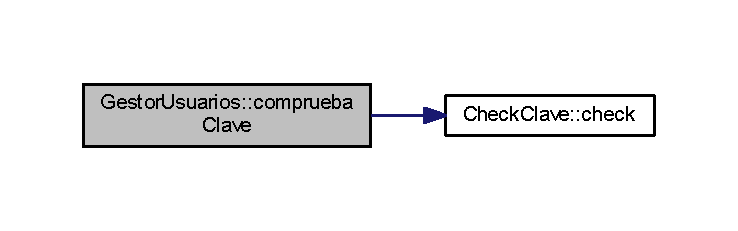
\includegraphics[width=350pt]{class_gestor_usuarios_a14c8dfce3dabbbdc4cd6214e6093ed60_cgraph}
\end{center}
\end{figure}




Here is the caller graph for this function\+:\nopagebreak
\begin{figure}[H]
\begin{center}
\leavevmode
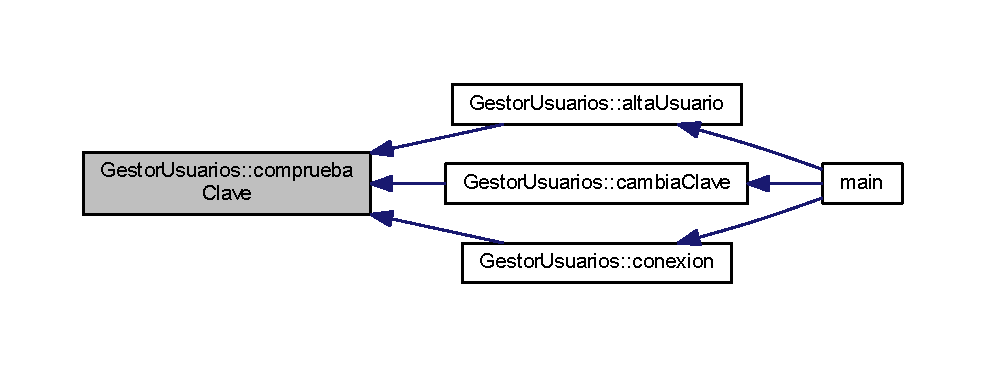
\includegraphics[width=350pt]{class_gestor_usuarios_a14c8dfce3dabbbdc4cd6214e6093ed60_icgraph}
\end{center}
\end{figure}


\index{Gestor\+Usuarios@{Gestor\+Usuarios}!conexion@{conexion}}
\index{conexion@{conexion}!Gestor\+Usuarios@{Gestor\+Usuarios}}
\subsubsection[{\texorpdfstring{conexion(string \&id, string \&clave)}{conexion(string &id, string &clave)}}]{\setlength{\rightskip}{0pt plus 5cm}void Gestor\+Usuarios\+::conexion (
\begin{DoxyParamCaption}
\item[{string \&}]{id, }
\item[{string \&}]{clave}
\end{DoxyParamCaption}
)}\hypertarget{class_gestor_usuarios_a3b929870c33c4864d3c1f32f2614a64d}{}\label{class_gestor_usuarios_a3b929870c33c4864d3c1f32f2614a64d}
To connect a user 
\begin{DoxyParams}{Parameters}
{\em id} & of the user \\
\hline
{\em clave} & key of the user \\
\hline
\end{DoxyParams}


Definition at line 159 of file Gestor\+Usuarios.\+cpp.



Here is the call graph for this function\+:\nopagebreak
\begin{figure}[H]
\begin{center}
\leavevmode
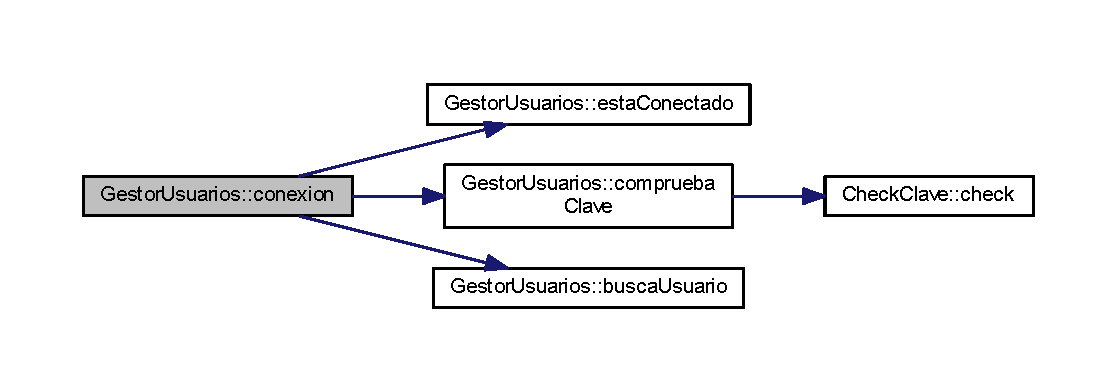
\includegraphics[width=350pt]{class_gestor_usuarios_a3b929870c33c4864d3c1f32f2614a64d_cgraph}
\end{center}
\end{figure}




Here is the caller graph for this function\+:\nopagebreak
\begin{figure}[H]
\begin{center}
\leavevmode
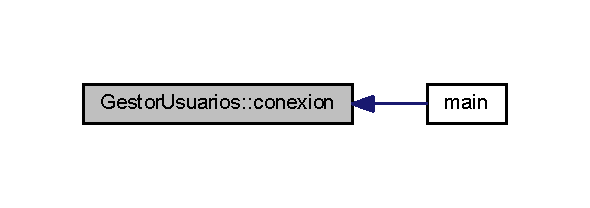
\includegraphics[width=283pt]{class_gestor_usuarios_a3b929870c33c4864d3c1f32f2614a64d_icgraph}
\end{center}
\end{figure}


\index{Gestor\+Usuarios@{Gestor\+Usuarios}!desconexion@{desconexion}}
\index{desconexion@{desconexion}!Gestor\+Usuarios@{Gestor\+Usuarios}}
\subsubsection[{\texorpdfstring{desconexion(string \&id)}{desconexion(string &id)}}]{\setlength{\rightskip}{0pt plus 5cm}void Gestor\+Usuarios\+::desconexion (
\begin{DoxyParamCaption}
\item[{string \&}]{id}
\end{DoxyParamCaption}
)}\hypertarget{class_gestor_usuarios_a1e57859037abf37a190ad2c60ed22f2b}{}\label{class_gestor_usuarios_a1e57859037abf37a190ad2c60ed22f2b}
To disconnect a user 
\begin{DoxyParams}{Parameters}
{\em id} & of the user \\
\hline
\end{DoxyParams}


Definition at line 184 of file Gestor\+Usuarios.\+cpp.



Here is the caller graph for this function\+:\nopagebreak
\begin{figure}[H]
\begin{center}
\leavevmode
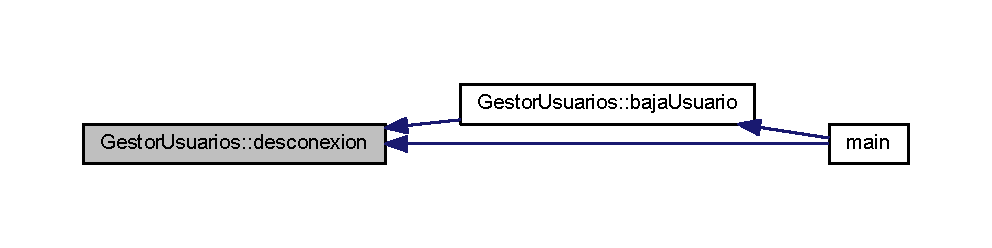
\includegraphics[width=350pt]{class_gestor_usuarios_a1e57859037abf37a190ad2c60ed22f2b_icgraph}
\end{center}
\end{figure}


\index{Gestor\+Usuarios@{Gestor\+Usuarios}!esta\+Conectado@{esta\+Conectado}}
\index{esta\+Conectado@{esta\+Conectado}!Gestor\+Usuarios@{Gestor\+Usuarios}}
\subsubsection[{\texorpdfstring{esta\+Conectado(string \&id)}{estaConectado(string &id)}}]{\setlength{\rightskip}{0pt plus 5cm}bool Gestor\+Usuarios\+::esta\+Conectado (
\begin{DoxyParamCaption}
\item[{string \&}]{id}
\end{DoxyParamCaption}
)}\hypertarget{class_gestor_usuarios_a41196c2a9b3abd71e7eb8f79fd765960}{}\label{class_gestor_usuarios_a41196c2a9b3abd71e7eb8f79fd765960}
To check if a user is connect 
\begin{DoxyParams}{Parameters}
{\em id} & of the user \\
\hline
\end{DoxyParams}
\begin{DoxyReturn}{Returns}
a boolean value (true if connect or false is not) 
\end{DoxyReturn}


Definition at line 198 of file Gestor\+Usuarios.\+cpp.



Here is the caller graph for this function\+:\nopagebreak
\begin{figure}[H]
\begin{center}
\leavevmode
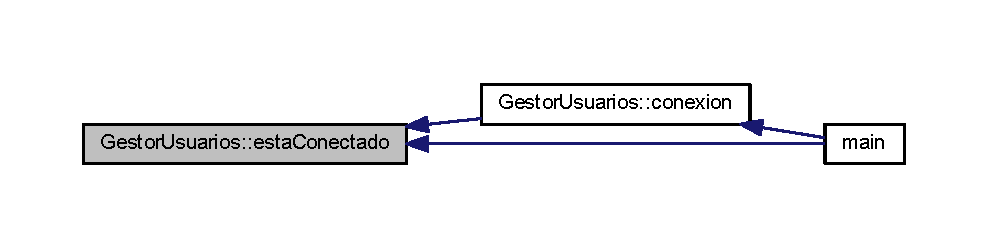
\includegraphics[width=350pt]{class_gestor_usuarios_a41196c2a9b3abd71e7eb8f79fd765960_icgraph}
\end{center}
\end{figure}


\index{Gestor\+Usuarios@{Gestor\+Usuarios}!operator=@{operator=}}
\index{operator=@{operator=}!Gestor\+Usuarios@{Gestor\+Usuarios}}
\subsubsection[{\texorpdfstring{operator=(\+Gestor\+Usuarios \&g)}{operator=(GestorUsuarios &g)}}]{\setlength{\rightskip}{0pt plus 5cm}{\bf Gestor\+Usuarios} \& Gestor\+Usuarios\+::operator= (
\begin{DoxyParamCaption}
\item[{{\bf Gestor\+Usuarios} \&}]{g}
\end{DoxyParamCaption}
)}\hypertarget{class_gestor_usuarios_abd8499f2178dc4e730674a78ecddae79}{}\label{class_gestor_usuarios_abd8499f2178dc4e730674a78ecddae79}
User manager operator= define operator = 
\begin{DoxyParams}{Parameters}
{\em g} & a user manager \\
\hline
\end{DoxyParams}
\begin{DoxyReturn}{Returns}

\end{DoxyReturn}


Definition at line 47 of file Gestor\+Usuarios.\+cpp.



Here is the call graph for this function\+:\nopagebreak
\begin{figure}[H]
\begin{center}
\leavevmode
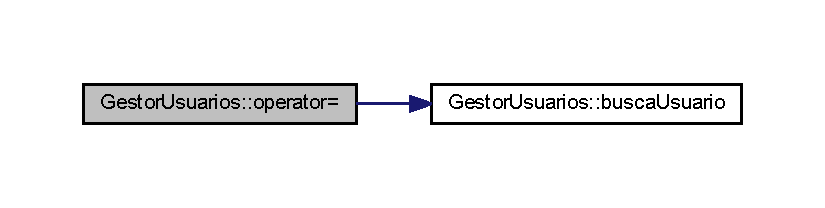
\includegraphics[width=350pt]{class_gestor_usuarios_abd8499f2178dc4e730674a78ecddae79_cgraph}
\end{center}
\end{figure}


\index{Gestor\+Usuarios@{Gestor\+Usuarios}!usuarios\+Conectados@{usuarios\+Conectados}}
\index{usuarios\+Conectados@{usuarios\+Conectados}!Gestor\+Usuarios@{Gestor\+Usuarios}}
\subsubsection[{\texorpdfstring{usuarios\+Conectados()}{usuariosConectados()}}]{\setlength{\rightskip}{0pt plus 5cm}set$<$ string $>$ Gestor\+Usuarios\+::usuarios\+Conectados (
\begin{DoxyParamCaption}
{}
\end{DoxyParamCaption}
)}\hypertarget{class_gestor_usuarios_a2a20b4c548e4bbe113174a416873194a}{}\label{class_gestor_usuarios_a2a20b4c548e4bbe113174a416873194a}
Show users connect \begin{DoxyReturn}{Returns}
a set of users 
\end{DoxyReturn}


Definition at line 207 of file Gestor\+Usuarios.\+cpp.



Here is the caller graph for this function\+:\nopagebreak
\begin{figure}[H]
\begin{center}
\leavevmode
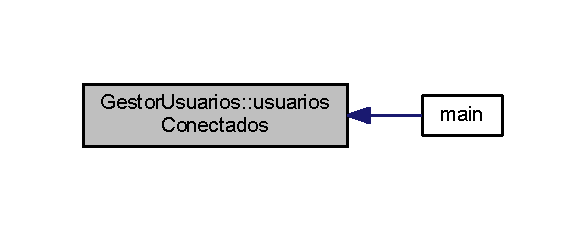
\includegraphics[width=281pt]{class_gestor_usuarios_a2a20b4c548e4bbe113174a416873194a_icgraph}
\end{center}
\end{figure}




The documentation for this class was generated from the following files\+:\begin{DoxyCompactItemize}
\item 
\hyperlink{_gestor_usuarios_8h}{Gestor\+Usuarios.\+h}\item 
\hyperlink{_gestor_usuarios_8cpp}{Gestor\+Usuarios.\+cpp}\end{DoxyCompactItemize}

\hypertarget{classpassword__not__accepted}{}\section{password\+\_\+not\+\_\+accepted Class Reference}
\label{classpassword__not__accepted}\index{password\+\_\+not\+\_\+accepted@{password\+\_\+not\+\_\+accepted}}


{\ttfamily \#include $<$password not accepted.\+h$>$}



Inheritance diagram for password\+\_\+not\+\_\+accepted\+:\nopagebreak
\begin{figure}[H]
\begin{center}
\leavevmode
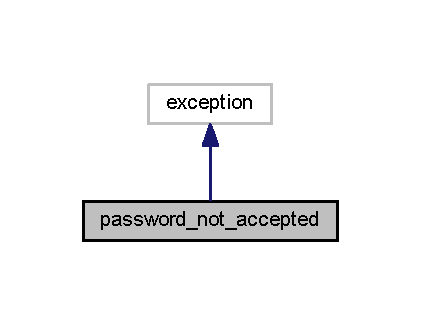
\includegraphics[width=202pt]{classpassword__not__accepted__inherit__graph}
\end{center}
\end{figure}


Collaboration diagram for password\+\_\+not\+\_\+accepted\+:\nopagebreak
\begin{figure}[H]
\begin{center}
\leavevmode
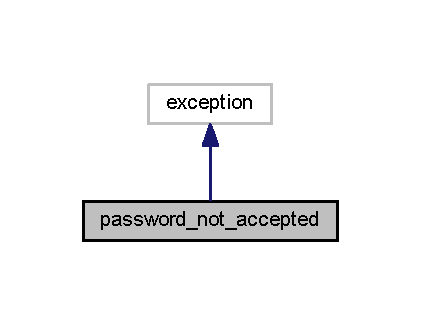
\includegraphics[width=202pt]{classpassword__not__accepted__coll__graph}
\end{center}
\end{figure}
\subsection*{Public Member Functions}
\begin{DoxyCompactItemize}
\item 
virtual const char $\ast$ \hyperlink{classpassword__not__accepted_a272c1e07f91db0e2661c272107dd4de8}{what} () const   throw ()
\item 
virtual \hyperlink{classpassword__not__accepted_a497f747f1453502ccee7076b669514c3}{$\sim$password\+\_\+not\+\_\+accepted} ()  throw ()
\end{DoxyCompactItemize}


\subsection{Detailed Description}
custom exception thrown when a password is not valid. 

Definition at line 18 of file password not accepted.\+h.



\subsection{Constructor \& Destructor Documentation}
\index{password\+\_\+not\+\_\+accepted@{password\+\_\+not\+\_\+accepted}!````~password\+\_\+not\+\_\+accepted@{$\sim$password\+\_\+not\+\_\+accepted}}
\index{````~password\+\_\+not\+\_\+accepted@{$\sim$password\+\_\+not\+\_\+accepted}!password\+\_\+not\+\_\+accepted@{password\+\_\+not\+\_\+accepted}}
\subsubsection[{\texorpdfstring{$\sim$password\+\_\+not\+\_\+accepted()}{~password_not_accepted()}}]{\setlength{\rightskip}{0pt plus 5cm}virtual password\+\_\+not\+\_\+accepted\+::$\sim$password\+\_\+not\+\_\+accepted (
\begin{DoxyParamCaption}
{}
\end{DoxyParamCaption}
) throw  ) \hspace{0.3cm}{\ttfamily [inline]}, {\ttfamily [virtual]}}\hypertarget{classpassword__not__accepted_a497f747f1453502ccee7076b669514c3}{}\label{classpassword__not__accepted_a497f747f1453502ccee7076b669514c3}
exception destructor. does nothing. 

Definition at line 32 of file password not accepted.\+h.



\subsection{Member Function Documentation}
\index{password\+\_\+not\+\_\+accepted@{password\+\_\+not\+\_\+accepted}!what@{what}}
\index{what@{what}!password\+\_\+not\+\_\+accepted@{password\+\_\+not\+\_\+accepted}}
\subsubsection[{\texorpdfstring{what() const }{what() const }}]{\setlength{\rightskip}{0pt plus 5cm}virtual const char$\ast$ password\+\_\+not\+\_\+accepted\+::what (
\begin{DoxyParamCaption}
{}
\end{DoxyParamCaption}
) const throw  ) \hspace{0.3cm}{\ttfamily [inline]}, {\ttfamily [virtual]}}\hypertarget{classpassword__not__accepted_a272c1e07f91db0e2661c272107dd4de8}{}\label{classpassword__not__accepted_a272c1e07f91db0e2661c272107dd4de8}
shows the exception information when called. In this case, the information is the string \char`\"{}\+Clave no valida\char`\"{}. 

Definition at line 24 of file password not accepted.\+h.



The documentation for this class was generated from the following file\+:\begin{DoxyCompactItemize}
\item 
\hyperlink{password_01not_01accepted_8h}{password not accepted.\+h}\end{DoxyCompactItemize}

\hypertarget{classuser__not__found}{}\section{user\+\_\+not\+\_\+found Class Reference}
\label{classuser__not__found}\index{user\+\_\+not\+\_\+found@{user\+\_\+not\+\_\+found}}


{\ttfamily \#include $<$user not found.\+h$>$}



Inheritance diagram for user\+\_\+not\+\_\+found\+:\nopagebreak
\begin{figure}[H]
\begin{center}
\leavevmode
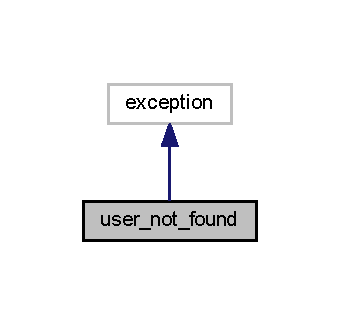
\includegraphics[width=163pt]{classuser__not__found__inherit__graph}
\end{center}
\end{figure}


Collaboration diagram for user\+\_\+not\+\_\+found\+:\nopagebreak
\begin{figure}[H]
\begin{center}
\leavevmode
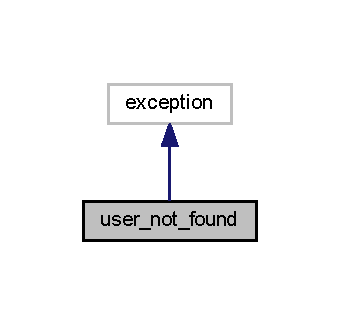
\includegraphics[width=163pt]{classuser__not__found__coll__graph}
\end{center}
\end{figure}
\subsection*{Public Member Functions}
\begin{DoxyCompactItemize}
\item 
virtual const char $\ast$ \hyperlink{classuser__not__found_a3c321063325306e880d515ea2994cd8b}{what} () const   throw ()
\item 
virtual \hyperlink{classuser__not__found_acc5145fbe86a9f9b7ad22f86b9e4a9fd}{$\sim$user\+\_\+not\+\_\+found} ()  throw ()
\end{DoxyCompactItemize}


\subsection{Detailed Description}
custom exception thrown in case of no user is found. 

Definition at line 19 of file user not found.\+h.



\subsection{Constructor \& Destructor Documentation}
\index{user\+\_\+not\+\_\+found@{user\+\_\+not\+\_\+found}!````~user\+\_\+not\+\_\+found@{$\sim$user\+\_\+not\+\_\+found}}
\index{````~user\+\_\+not\+\_\+found@{$\sim$user\+\_\+not\+\_\+found}!user\+\_\+not\+\_\+found@{user\+\_\+not\+\_\+found}}
\subsubsection[{\texorpdfstring{$\sim$user\+\_\+not\+\_\+found()}{~user_not_found()}}]{\setlength{\rightskip}{0pt plus 5cm}virtual user\+\_\+not\+\_\+found\+::$\sim$user\+\_\+not\+\_\+found (
\begin{DoxyParamCaption}
{}
\end{DoxyParamCaption}
) throw  ) \hspace{0.3cm}{\ttfamily [inline]}, {\ttfamily [virtual]}}\hypertarget{classuser__not__found_acc5145fbe86a9f9b7ad22f86b9e4a9fd}{}\label{classuser__not__found_acc5145fbe86a9f9b7ad22f86b9e4a9fd}
exception destructor. does nothing. 

Definition at line 33 of file user not found.\+h.



\subsection{Member Function Documentation}
\index{user\+\_\+not\+\_\+found@{user\+\_\+not\+\_\+found}!what@{what}}
\index{what@{what}!user\+\_\+not\+\_\+found@{user\+\_\+not\+\_\+found}}
\subsubsection[{\texorpdfstring{what() const }{what() const }}]{\setlength{\rightskip}{0pt plus 5cm}virtual const char$\ast$ user\+\_\+not\+\_\+found\+::what (
\begin{DoxyParamCaption}
{}
\end{DoxyParamCaption}
) const throw  ) \hspace{0.3cm}{\ttfamily [inline]}, {\ttfamily [virtual]}}\hypertarget{classuser__not__found_a3c321063325306e880d515ea2994cd8b}{}\label{classuser__not__found_a3c321063325306e880d515ea2994cd8b}
shows the exception information when called. In this case, the information is the string \char`\"{}\+Usuario no encontrado\char`\"{}. 

Definition at line 25 of file user not found.\+h.



The documentation for this class was generated from the following file\+:\begin{DoxyCompactItemize}
\item 
\hyperlink{user_01not_01found_8h}{user not found.\+h}\end{DoxyCompactItemize}

\hypertarget{class_usuario}{}\section{Usuario Class Reference}
\label{class_usuario}\index{Usuario@{Usuario}}


{\ttfamily \#include $<$Usuario.\+h$>$}

\subsection*{Public Member Functions}
\begin{DoxyCompactItemize}
\item 
\hyperlink{class_usuario_aa85a5371a098dfba5449140d9b8a472f}{Usuario} ()
\item 
\hyperlink{class_usuario_a305eda14decabbd02a61ed4154ea26b9}{Usuario} (string id, string clave, string nombre)
\item 
\hyperlink{class_usuario_a5b8c44d4b7d7b2e49542cda79521fffa}{Usuario} (const \hyperlink{class_usuario}{Usuario} \&orig)
\item 
virtual \hyperlink{class_usuario_ab4096b0b8300ecb47b10c555fb09c997}{$\sim$\+Usuario} ()
\item 
string \hyperlink{class_usuario_aceb0e105938da68e83cfa8f45ec41487}{get\+Id} ()
\item 
string \hyperlink{class_usuario_a322129e7a34d7b332af4dfa13a4fb8d9}{get\+Clave} ()
\item 
string \hyperlink{class_usuario_a2fb6b8343b535d8c42f62bda587e58d0}{get\+Nombre} ()
\item 
void \hyperlink{class_usuario_a74ba4e76654f3ebabb2bd51f3a748b41}{set\+Clave} (string \&clave)
\item 
string \hyperlink{class_usuario_a5f2234908325bc89b0849c0ab28d61aa}{to\+String} ()
\item 
void \hyperlink{class_usuario_a62f031d10687b259237ca038725c82da}{set\+Nombre} (string \&nombre)
\item 
void \hyperlink{class_usuario_a567493e3fee3c245fee24db39f8d0e32}{set\+Id} (string \&id)
\end{DoxyCompactItemize}


\subsection{Detailed Description}
class representing an user, with an unique id, name and password. 

Definition at line 17 of file Usuario.\+h.



\subsection{Constructor \& Destructor Documentation}
\index{Usuario@{Usuario}!Usuario@{Usuario}}
\index{Usuario@{Usuario}!Usuario@{Usuario}}
\subsubsection[{\texorpdfstring{Usuario()}{Usuario()}}]{\setlength{\rightskip}{0pt plus 5cm}Usuario\+::\+Usuario (
\begin{DoxyParamCaption}
{}
\end{DoxyParamCaption}
)}\hypertarget{class_usuario_aa85a5371a098dfba5449140d9b8a472f}{}\label{class_usuario_aa85a5371a098dfba5449140d9b8a472f}
user default constructor. sets all variables class members to null. 

Definition at line 15 of file Usuario.\+cpp.

\index{Usuario@{Usuario}!Usuario@{Usuario}}
\index{Usuario@{Usuario}!Usuario@{Usuario}}
\subsubsection[{\texorpdfstring{Usuario(string id, string clave, string nombre)}{Usuario(string id, string clave, string nombre)}}]{\setlength{\rightskip}{0pt plus 5cm}Usuario\+::\+Usuario (
\begin{DoxyParamCaption}
\item[{string}]{id, }
\item[{string}]{clave, }
\item[{string}]{nombre}
\end{DoxyParamCaption}
)}\hypertarget{class_usuario_a305eda14decabbd02a61ed4154ea26b9}{}\label{class_usuario_a305eda14decabbd02a61ed4154ea26b9}
user constructor with parameters. set the variables with the values passed. 
\begin{DoxyParams}{Parameters}
{\em id} & the user id. \\
\hline
{\em clave} & the user password. \\
\hline
{\em nombre} & the name of the user. \\
\hline
\end{DoxyParams}


Definition at line 28 of file Usuario.\+cpp.

\index{Usuario@{Usuario}!Usuario@{Usuario}}
\index{Usuario@{Usuario}!Usuario@{Usuario}}
\subsubsection[{\texorpdfstring{Usuario(const Usuario \&orig)}{Usuario(const Usuario &orig)}}]{\setlength{\rightskip}{0pt plus 5cm}Usuario\+::\+Usuario (
\begin{DoxyParamCaption}
\item[{const {\bf Usuario} \&}]{orig}
\end{DoxyParamCaption}
)}\hypertarget{class_usuario_a5b8c44d4b7d7b2e49542cda79521fffa}{}\label{class_usuario_a5b8c44d4b7d7b2e49542cda79521fffa}
user copy constructor. 
\begin{DoxyParams}{Parameters}
{\em orig} & user to copy. \\
\hline
\end{DoxyParams}


Definition at line 38 of file Usuario.\+cpp.

\index{Usuario@{Usuario}!````~Usuario@{$\sim$\+Usuario}}
\index{````~Usuario@{$\sim$\+Usuario}!Usuario@{Usuario}}
\subsubsection[{\texorpdfstring{$\sim$\+Usuario()}{~Usuario()}}]{\setlength{\rightskip}{0pt plus 5cm}Usuario\+::$\sim$\+Usuario (
\begin{DoxyParamCaption}
{}
\end{DoxyParamCaption}
)\hspace{0.3cm}{\ttfamily [virtual]}}\hypertarget{class_usuario_ab4096b0b8300ecb47b10c555fb09c997}{}\label{class_usuario_ab4096b0b8300ecb47b10c555fb09c997}
user destructor. does nothing for now. 

Definition at line 48 of file Usuario.\+cpp.



\subsection{Member Function Documentation}
\index{Usuario@{Usuario}!get\+Clave@{get\+Clave}}
\index{get\+Clave@{get\+Clave}!Usuario@{Usuario}}
\subsubsection[{\texorpdfstring{get\+Clave()}{getClave()}}]{\setlength{\rightskip}{0pt plus 5cm}string Usuario\+::get\+Clave (
\begin{DoxyParamCaption}
{}
\end{DoxyParamCaption}
)}\hypertarget{class_usuario_a322129e7a34d7b332af4dfa13a4fb8d9}{}\label{class_usuario_a322129e7a34d7b332af4dfa13a4fb8d9}
return the user password. \begin{DoxyReturn}{Returns}
user password. 
\end{DoxyReturn}


Definition at line 63 of file Usuario.\+cpp.



Here is the caller graph for this function\+:\nopagebreak
\begin{figure}[H]
\begin{center}
\leavevmode
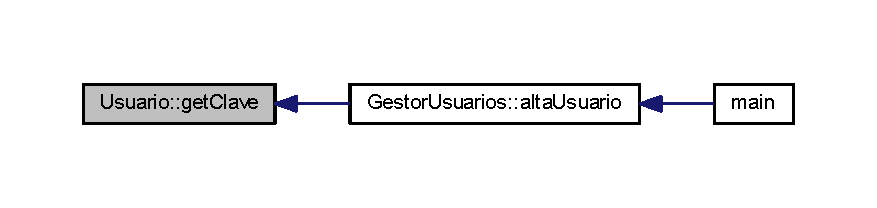
\includegraphics[width=350pt]{class_usuario_a322129e7a34d7b332af4dfa13a4fb8d9_icgraph}
\end{center}
\end{figure}


\index{Usuario@{Usuario}!get\+Id@{get\+Id}}
\index{get\+Id@{get\+Id}!Usuario@{Usuario}}
\subsubsection[{\texorpdfstring{get\+Id()}{getId()}}]{\setlength{\rightskip}{0pt plus 5cm}string Usuario\+::get\+Id (
\begin{DoxyParamCaption}
{}
\end{DoxyParamCaption}
)}\hypertarget{class_usuario_aceb0e105938da68e83cfa8f45ec41487}{}\label{class_usuario_aceb0e105938da68e83cfa8f45ec41487}
return the user id. \begin{DoxyReturn}{Returns}
user id. 
\end{DoxyReturn}


Definition at line 55 of file Usuario.\+cpp.



Here is the caller graph for this function\+:\nopagebreak
\begin{figure}[H]
\begin{center}
\leavevmode
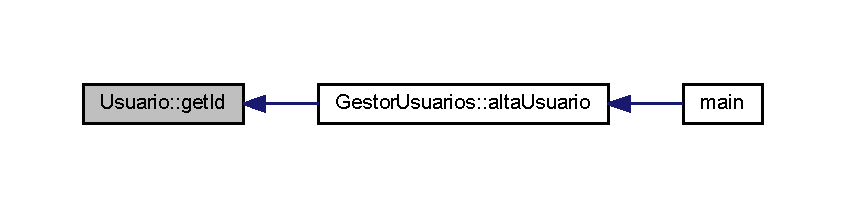
\includegraphics[width=350pt]{class_usuario_aceb0e105938da68e83cfa8f45ec41487_icgraph}
\end{center}
\end{figure}


\index{Usuario@{Usuario}!get\+Nombre@{get\+Nombre}}
\index{get\+Nombre@{get\+Nombre}!Usuario@{Usuario}}
\subsubsection[{\texorpdfstring{get\+Nombre()}{getNombre()}}]{\setlength{\rightskip}{0pt plus 5cm}string Usuario\+::get\+Nombre (
\begin{DoxyParamCaption}
{}
\end{DoxyParamCaption}
)}\hypertarget{class_usuario_a2fb6b8343b535d8c42f62bda587e58d0}{}\label{class_usuario_a2fb6b8343b535d8c42f62bda587e58d0}
return the user name. \begin{DoxyReturn}{Returns}
user name. 
\end{DoxyReturn}


Definition at line 71 of file Usuario.\+cpp.

\index{Usuario@{Usuario}!set\+Clave@{set\+Clave}}
\index{set\+Clave@{set\+Clave}!Usuario@{Usuario}}
\subsubsection[{\texorpdfstring{set\+Clave(string \&clave)}{setClave(string &clave)}}]{\setlength{\rightskip}{0pt plus 5cm}void Usuario\+::set\+Clave (
\begin{DoxyParamCaption}
\item[{string \&}]{clave}
\end{DoxyParamCaption}
)}\hypertarget{class_usuario_a74ba4e76654f3ebabb2bd51f3a748b41}{}\label{class_usuario_a74ba4e76654f3ebabb2bd51f3a748b41}
set the user password. 
\begin{DoxyParams}{Parameters}
{\em clave} & the new password. \\
\hline
\end{DoxyParams}


Definition at line 79 of file Usuario.\+cpp.



Here is the caller graph for this function\+:\nopagebreak
\begin{figure}[H]
\begin{center}
\leavevmode
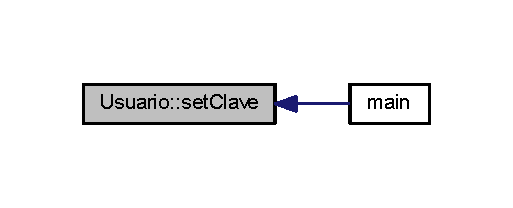
\includegraphics[width=246pt]{class_usuario_a74ba4e76654f3ebabb2bd51f3a748b41_icgraph}
\end{center}
\end{figure}


\index{Usuario@{Usuario}!set\+Id@{set\+Id}}
\index{set\+Id@{set\+Id}!Usuario@{Usuario}}
\subsubsection[{\texorpdfstring{set\+Id(string \&id)}{setId(string &id)}}]{\setlength{\rightskip}{0pt plus 5cm}void Usuario\+::set\+Id (
\begin{DoxyParamCaption}
\item[{string \&}]{id}
\end{DoxyParamCaption}
)}\hypertarget{class_usuario_a567493e3fee3c245fee24db39f8d0e32}{}\label{class_usuario_a567493e3fee3c245fee24db39f8d0e32}
set the user id. 
\begin{DoxyParams}{Parameters}
{\em id} & the new id. \\
\hline
\end{DoxyParams}


Definition at line 105 of file Usuario.\+cpp.



Here is the caller graph for this function\+:\nopagebreak
\begin{figure}[H]
\begin{center}
\leavevmode
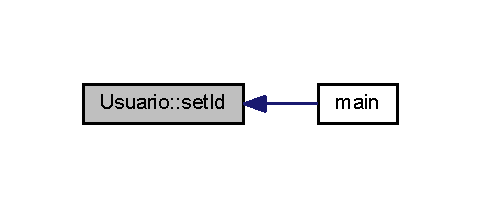
\includegraphics[width=231pt]{class_usuario_a567493e3fee3c245fee24db39f8d0e32_icgraph}
\end{center}
\end{figure}


\index{Usuario@{Usuario}!set\+Nombre@{set\+Nombre}}
\index{set\+Nombre@{set\+Nombre}!Usuario@{Usuario}}
\subsubsection[{\texorpdfstring{set\+Nombre(string \&nombre)}{setNombre(string &nombre)}}]{\setlength{\rightskip}{0pt plus 5cm}void Usuario\+::set\+Nombre (
\begin{DoxyParamCaption}
\item[{string \&}]{nombre}
\end{DoxyParamCaption}
)}\hypertarget{class_usuario_a62f031d10687b259237ca038725c82da}{}\label{class_usuario_a62f031d10687b259237ca038725c82da}
set the user name. 
\begin{DoxyParams}{Parameters}
{\em nombre} & the new name. \\
\hline
\end{DoxyParams}


Definition at line 97 of file Usuario.\+cpp.



Here is the caller graph for this function\+:\nopagebreak
\begin{figure}[H]
\begin{center}
\leavevmode
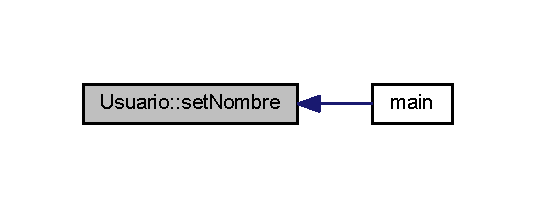
\includegraphics[width=257pt]{class_usuario_a62f031d10687b259237ca038725c82da_icgraph}
\end{center}
\end{figure}


\index{Usuario@{Usuario}!to\+String@{to\+String}}
\index{to\+String@{to\+String}!Usuario@{Usuario}}
\subsubsection[{\texorpdfstring{to\+String()}{toString()}}]{\setlength{\rightskip}{0pt plus 5cm}string Usuario\+::to\+String (
\begin{DoxyParamCaption}
{}
\end{DoxyParamCaption}
)}\hypertarget{class_usuario_a5f2234908325bc89b0849c0ab28d61aa}{}\label{class_usuario_a5f2234908325bc89b0849c0ab28d61aa}
allow to print user information. \begin{DoxyReturn}{Returns}
the string \char`\"{}user.\+id, user.\+password, user.\+name\char`\"{}. 
\end{DoxyReturn}


Definition at line 87 of file Usuario.\+cpp.



Here is the caller graph for this function\+:\nopagebreak
\begin{figure}[H]
\begin{center}
\leavevmode
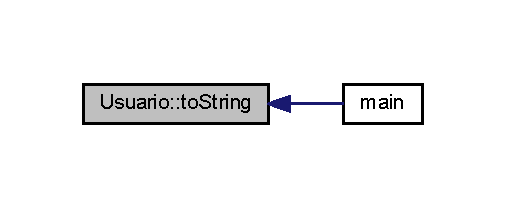
\includegraphics[width=243pt]{class_usuario_a5f2234908325bc89b0849c0ab28d61aa_icgraph}
\end{center}
\end{figure}




The documentation for this class was generated from the following files\+:\begin{DoxyCompactItemize}
\item 
\hyperlink{_usuario_8h}{Usuario.\+h}\item 
\hyperlink{_usuario_8cpp}{Usuario.\+cpp}\end{DoxyCompactItemize}

\chapter{File Documentation}
\hypertarget{_check_clave_8cpp}{}\section{Check\+Clave.\+cpp File Reference}
\label{_check_clave_8cpp}\index{Check\+Clave.\+cpp@{Check\+Clave.\+cpp}}
{\ttfamily \#include \char`\"{}Check\+Clave.\+h\char`\"{}}\\*
{\ttfamily \#include $<$fstream$>$}\\*
{\ttfamily \#include \char`\"{}file not found.\+h\char`\"{}}\\*
{\ttfamily \#include $<$iostream$>$}\\*
Include dependency graph for Check\+Clave.\+cpp\+:\nopagebreak
\begin{figure}[H]
\begin{center}
\leavevmode
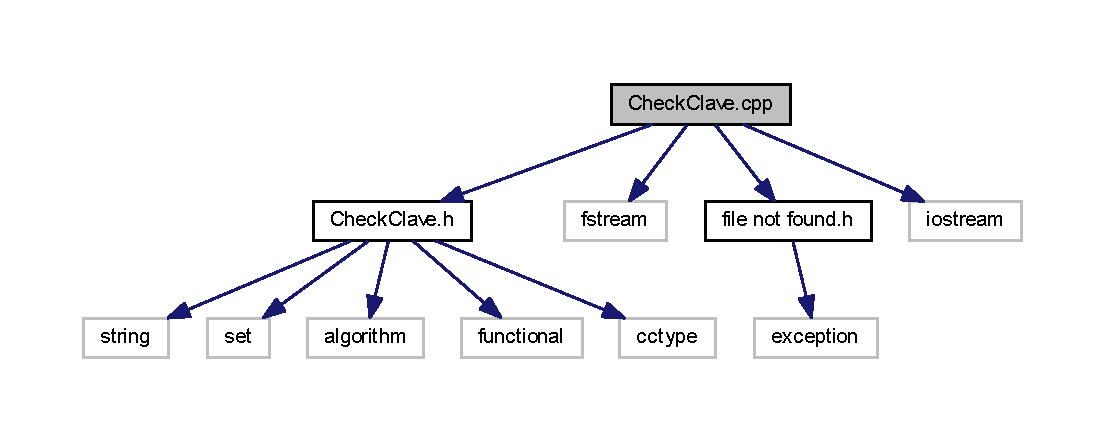
\includegraphics[width=350pt]{_check_clave_8cpp__incl}
\end{center}
\end{figure}

\hypertarget{_check_clave_8h}{}\section{Check\+Clave.\+h File Reference}
\label{_check_clave_8h}\index{Check\+Clave.\+h@{Check\+Clave.\+h}}
{\ttfamily \#include $<$string$>$}\\*
{\ttfamily \#include $<$set$>$}\\*
{\ttfamily \#include $<$algorithm$>$}\\*
{\ttfamily \#include $<$functional$>$}\\*
{\ttfamily \#include $<$cctype$>$}\\*
Include dependency graph for Check\+Clave.\+h\+:\nopagebreak
\begin{figure}[H]
\begin{center}
\leavevmode
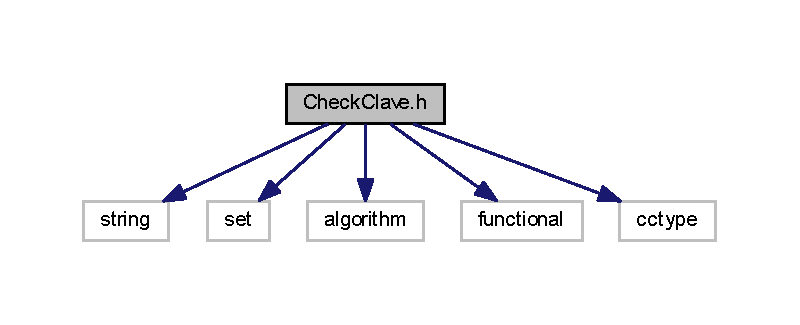
\includegraphics[width=350pt]{_check_clave_8h__incl}
\end{center}
\end{figure}
This graph shows which files directly or indirectly include this file\+:\nopagebreak
\begin{figure}[H]
\begin{center}
\leavevmode
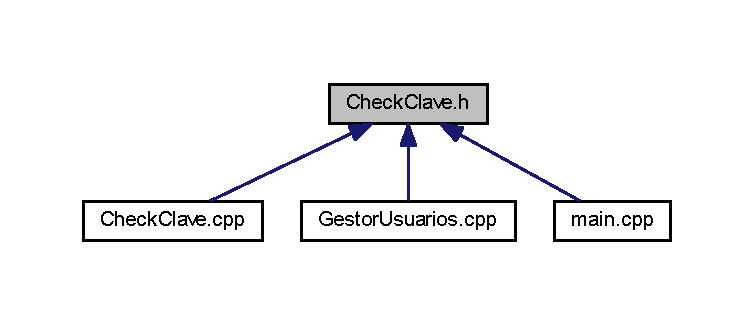
\includegraphics[width=350pt]{_check_clave_8h__dep__incl}
\end{center}
\end{figure}
\subsection*{Classes}
\begin{DoxyCompactItemize}
\item 
class \hyperlink{class_check_clave}{Check\+Clave}
\end{DoxyCompactItemize}

\hypertarget{existing_01user_8h}{}\section{existing user.\+h File Reference}
\label{existing_01user_8h}\index{existing user.\+h@{existing user.\+h}}
{\ttfamily \#include $<$exception$>$}\\*
Include dependency graph for existing user.\+h\+:\nopagebreak
\begin{figure}[H]
\begin{center}
\leavevmode
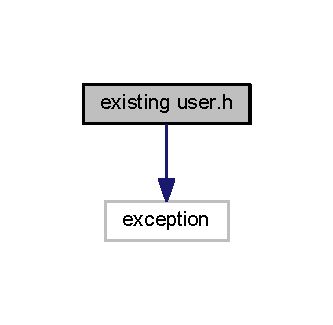
\includegraphics[width=160pt]{existing_01user_8h__incl}
\end{center}
\end{figure}
This graph shows which files directly or indirectly include this file\+:\nopagebreak
\begin{figure}[H]
\begin{center}
\leavevmode
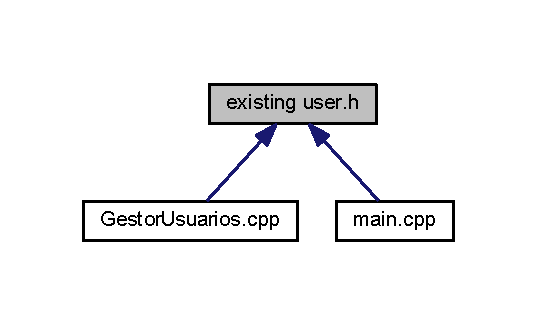
\includegraphics[width=258pt]{existing_01user_8h__dep__incl}
\end{center}
\end{figure}
\subsection*{Classes}
\begin{DoxyCompactItemize}
\item 
class \hyperlink{classexisting__user}{existing\+\_\+user}
\end{DoxyCompactItemize}

\hypertarget{file_01not_01found_8h}{}\section{file not found.\+h File Reference}
\label{file_01not_01found_8h}\index{file not found.\+h@{file not found.\+h}}
{\ttfamily \#include $<$exception$>$}\\*
Include dependency graph for file not found.\+h\+:\nopagebreak
\begin{figure}[H]
\begin{center}
\leavevmode
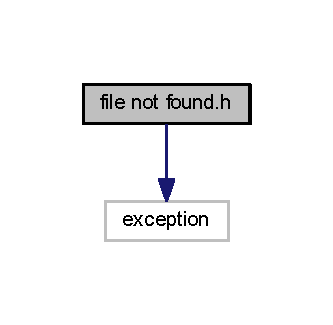
\includegraphics[width=160pt]{file_01not_01found_8h__incl}
\end{center}
\end{figure}
This graph shows which files directly or indirectly include this file\+:\nopagebreak
\begin{figure}[H]
\begin{center}
\leavevmode
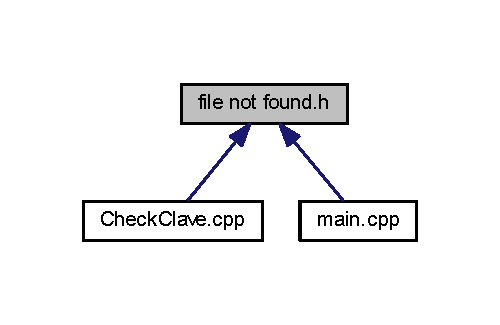
\includegraphics[width=240pt]{file_01not_01found_8h__dep__incl}
\end{center}
\end{figure}
\subsection*{Classes}
\begin{DoxyCompactItemize}
\item 
class \hyperlink{classfile__not__found}{file\+\_\+not\+\_\+found}
\end{DoxyCompactItemize}

\hypertarget{_gestor_usuarios_8cpp}{}\section{Gestor\+Usuarios.\+cpp File Reference}
\label{_gestor_usuarios_8cpp}\index{Gestor\+Usuarios.\+cpp@{Gestor\+Usuarios.\+cpp}}
{\ttfamily \#include \char`\"{}Gestor\+Usuarios.\+h\char`\"{}}\\*
{\ttfamily \#include $<$iostream$>$}\\*
{\ttfamily \#include \char`\"{}Check\+Clave.\+h\char`\"{}}\\*
{\ttfamily \#include \char`\"{}existing user.\+h\char`\"{}}\\*
{\ttfamily \#include \char`\"{}password not accepted.\+h\char`\"{}}\\*
{\ttfamily \#include \char`\"{}user not found.\+h\char`\"{}}\\*
Include dependency graph for Gestor\+Usuarios.\+cpp\+:\nopagebreak
\begin{figure}[H]
\begin{center}
\leavevmode
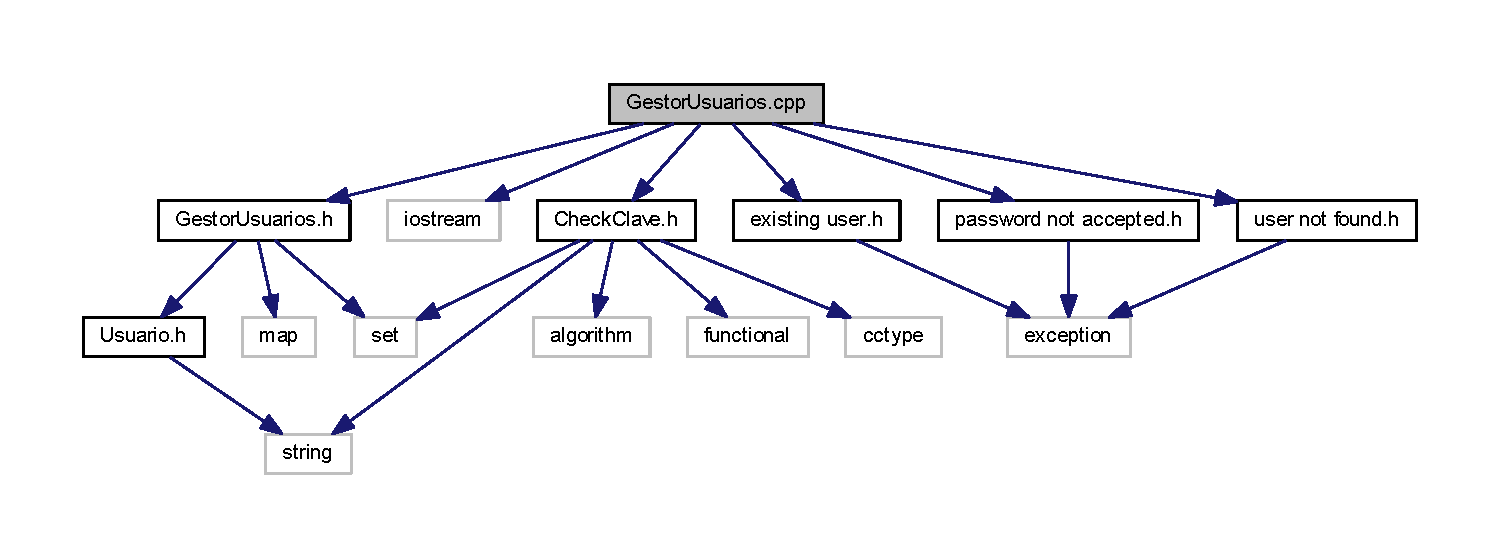
\includegraphics[width=350pt]{_gestor_usuarios_8cpp__incl}
\end{center}
\end{figure}

\hypertarget{_gestor_usuarios_8h}{}\section{Gestor\+Usuarios.\+h File Reference}
\label{_gestor_usuarios_8h}\index{Gestor\+Usuarios.\+h@{Gestor\+Usuarios.\+h}}
{\ttfamily \#include \char`\"{}Usuario.\+h\char`\"{}}\\*
{\ttfamily \#include $<$map$>$}\\*
{\ttfamily \#include $<$set$>$}\\*
Include dependency graph for Gestor\+Usuarios.\+h\+:\nopagebreak
\begin{figure}[H]
\begin{center}
\leavevmode
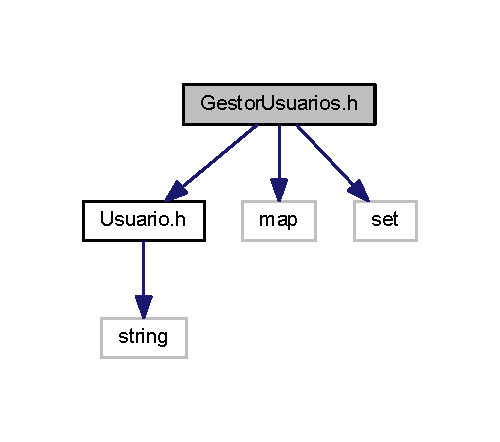
\includegraphics[width=240pt]{_gestor_usuarios_8h__incl}
\end{center}
\end{figure}
This graph shows which files directly or indirectly include this file\+:\nopagebreak
\begin{figure}[H]
\begin{center}
\leavevmode
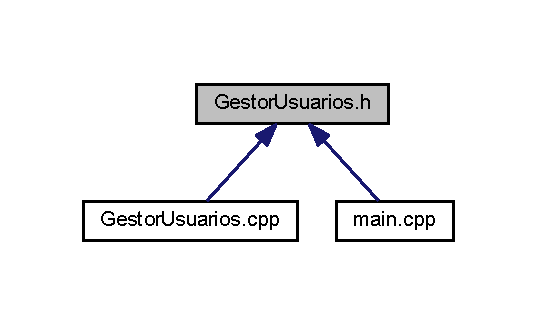
\includegraphics[width=258pt]{_gestor_usuarios_8h__dep__incl}
\end{center}
\end{figure}
\subsection*{Classes}
\begin{DoxyCompactItemize}
\item 
class \hyperlink{class_gestor_usuarios}{Gestor\+Usuarios}
\end{DoxyCompactItemize}

\hypertarget{main_8cpp}{}\section{main.\+cpp File Reference}
\label{main_8cpp}\index{main.\+cpp@{main.\+cpp}}
{\ttfamily \#include $<$cstdlib$>$}\\*
{\ttfamily \#include $<$iostream$>$}\\*
{\ttfamily \#include \char`\"{}Check\+Clave.\+h\char`\"{}}\\*
{\ttfamily \#include \char`\"{}Usuario.\+h\char`\"{}}\\*
{\ttfamily \#include \char`\"{}Gestor\+Usuarios.\+h\char`\"{}}\\*
{\ttfamily \#include \char`\"{}file not found.\+h\char`\"{}}\\*
{\ttfamily \#include \char`\"{}existing user.\+h\char`\"{}}\\*
{\ttfamily \#include \char`\"{}password not accepted.\+h\char`\"{}}\\*
{\ttfamily \#include \char`\"{}user not found.\+h\char`\"{}}\\*
Include dependency graph for main.\+cpp\+:\nopagebreak
\begin{figure}[H]
\begin{center}
\leavevmode
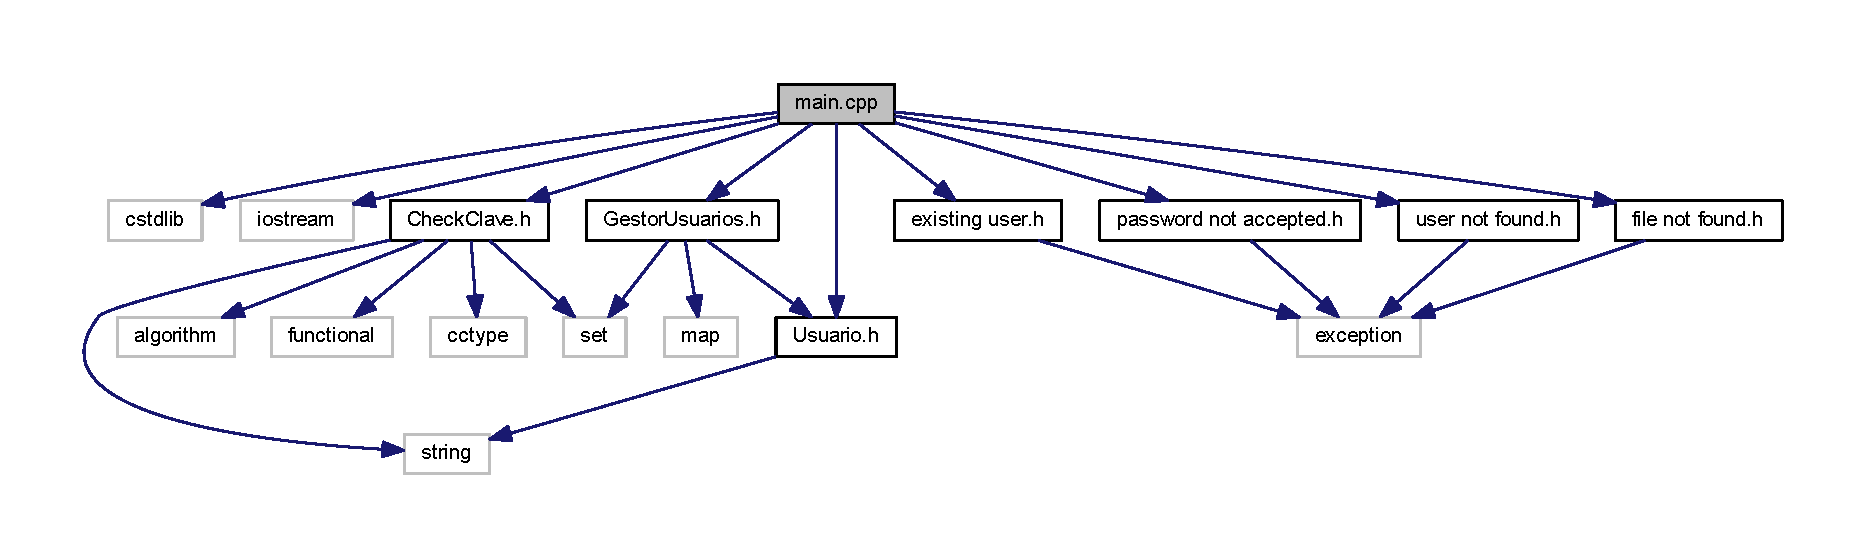
\includegraphics[width=350pt]{main_8cpp__incl}
\end{center}
\end{figure}
\subsection*{Functions}
\begin{DoxyCompactItemize}
\item 
int \hyperlink{main_8cpp_a3c04138a5bfe5d72780bb7e82a18e627}{main} (int argc, char $\ast$$\ast$argv)
\end{DoxyCompactItemize}


\subsection{Function Documentation}
\index{main.\+cpp@{main.\+cpp}!main@{main}}
\index{main@{main}!main.\+cpp@{main.\+cpp}}
\subsubsection[{\texorpdfstring{main(int argc, char $\ast$$\ast$argv)}{main(int argc, char **argv)}}]{\setlength{\rightskip}{0pt plus 5cm}int main (
\begin{DoxyParamCaption}
\item[{int}]{argc, }
\item[{char $\ast$$\ast$}]{argv}
\end{DoxyParamCaption}
)}\hypertarget{main_8cpp_a3c04138a5bfe5d72780bb7e82a18e627}{}\label{main_8cpp_a3c04138a5bfe5d72780bb7e82a18e627}


Definition at line 23 of file main.\+cpp.



Here is the call graph for this function\+:\nopagebreak
\begin{figure}[H]
\begin{center}
\leavevmode
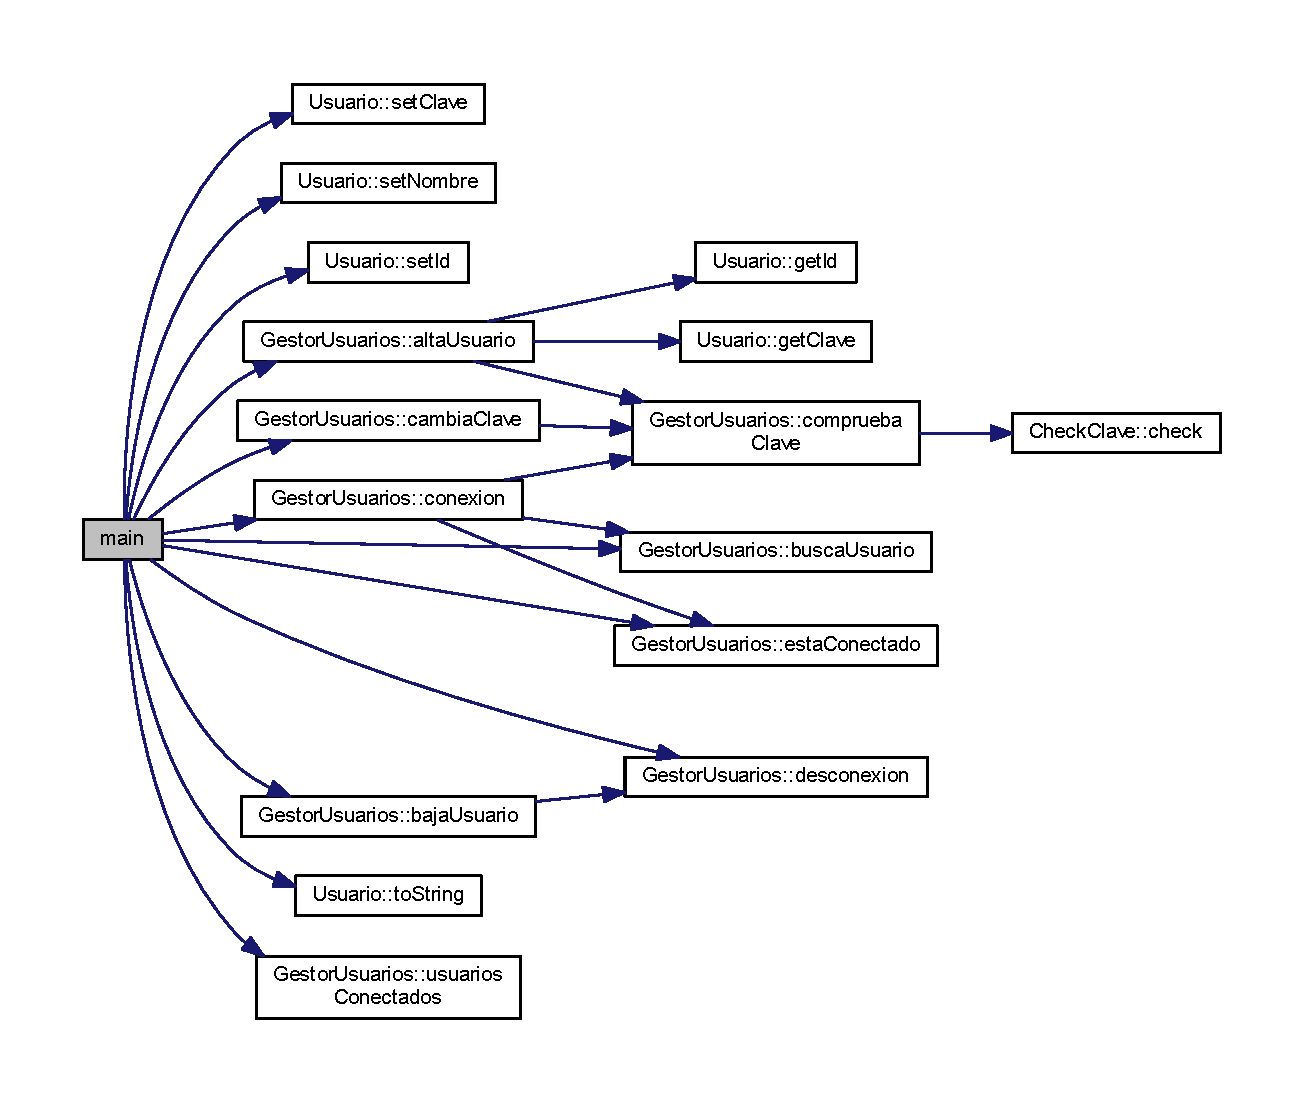
\includegraphics[width=350pt]{main_8cpp_a3c04138a5bfe5d72780bb7e82a18e627_cgraph}
\end{center}
\end{figure}



\hypertarget{password_01not_01accepted_8h}{}\section{password not accepted.\+h File Reference}
\label{password_01not_01accepted_8h}\index{password not accepted.\+h@{password not accepted.\+h}}
{\ttfamily \#include $<$exception$>$}\\*
Include dependency graph for password not accepted.\+h\+:\nopagebreak
\begin{figure}[H]
\begin{center}
\leavevmode
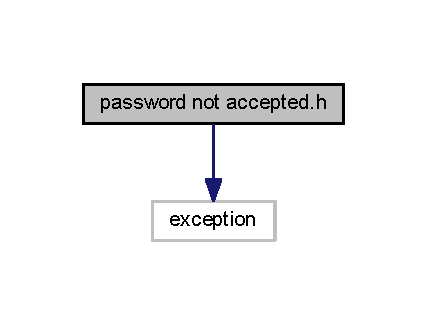
\includegraphics[width=205pt]{password_01not_01accepted_8h__incl}
\end{center}
\end{figure}
This graph shows which files directly or indirectly include this file\+:\nopagebreak
\begin{figure}[H]
\begin{center}
\leavevmode
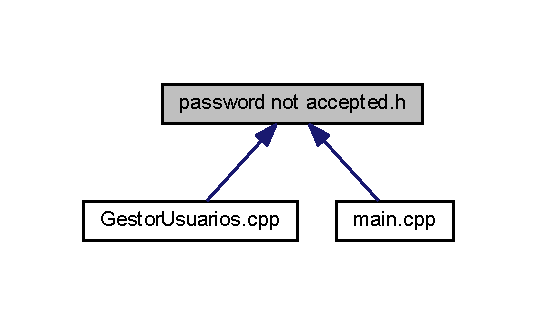
\includegraphics[width=258pt]{password_01not_01accepted_8h__dep__incl}
\end{center}
\end{figure}
\subsection*{Classes}
\begin{DoxyCompactItemize}
\item 
class \hyperlink{classpassword__not__accepted}{password\+\_\+not\+\_\+accepted}
\end{DoxyCompactItemize}

\hypertarget{user_01not_01found_8h}{}\section{user not found.\+h File Reference}
\label{user_01not_01found_8h}\index{user not found.\+h@{user not found.\+h}}
{\ttfamily \#include $<$exception$>$}\\*
Include dependency graph for user not found.\+h\+:\nopagebreak
\begin{figure}[H]
\begin{center}
\leavevmode
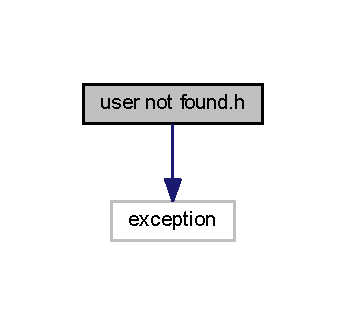
\includegraphics[width=166pt]{user_01not_01found_8h__incl}
\end{center}
\end{figure}
This graph shows which files directly or indirectly include this file\+:\nopagebreak
\begin{figure}[H]
\begin{center}
\leavevmode
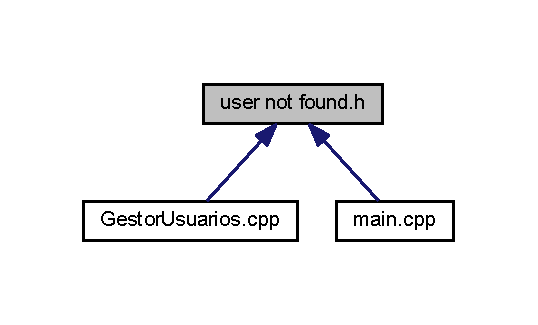
\includegraphics[width=258pt]{user_01not_01found_8h__dep__incl}
\end{center}
\end{figure}
\subsection*{Classes}
\begin{DoxyCompactItemize}
\item 
class \hyperlink{classuser__not__found}{user\+\_\+not\+\_\+found}
\end{DoxyCompactItemize}

\hypertarget{_usuario_8cpp}{}\section{Usuario.\+cpp File Reference}
\label{_usuario_8cpp}\index{Usuario.\+cpp@{Usuario.\+cpp}}
{\ttfamily \#include $<$sstream$>$}\\*
{\ttfamily \#include \char`\"{}Usuario.\+h\char`\"{}}\\*
Include dependency graph for Usuario.\+cpp\+:\nopagebreak
\begin{figure}[H]
\begin{center}
\leavevmode
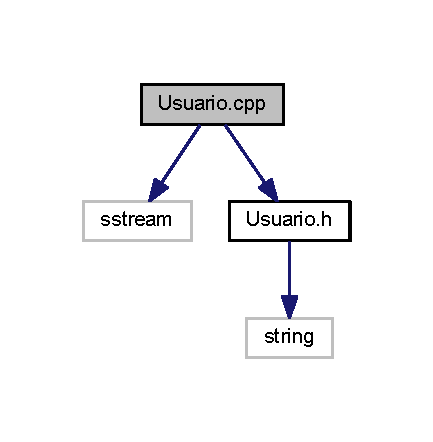
\includegraphics[width=208pt]{_usuario_8cpp__incl}
\end{center}
\end{figure}

\hypertarget{_usuario_8h}{}\section{Usuario.\+h File Reference}
\label{_usuario_8h}\index{Usuario.\+h@{Usuario.\+h}}
{\ttfamily \#include $<$string$>$}\\*
Include dependency graph for Usuario.\+h\+:\nopagebreak
\begin{figure}[H]
\begin{center}
\leavevmode
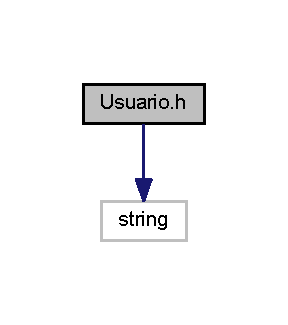
\includegraphics[width=138pt]{_usuario_8h__incl}
\end{center}
\end{figure}
This graph shows which files directly or indirectly include this file\+:\nopagebreak
\begin{figure}[H]
\begin{center}
\leavevmode
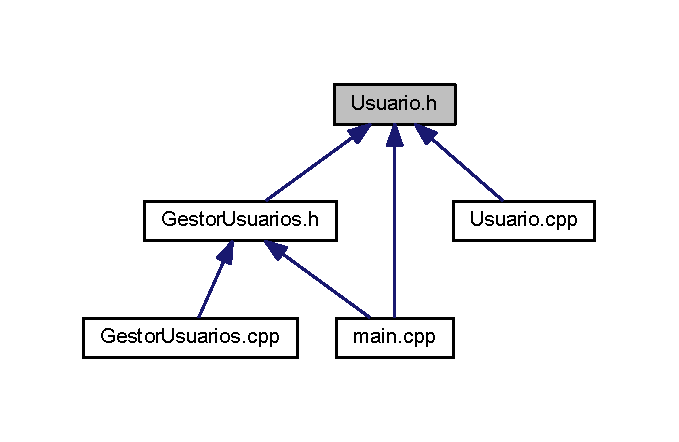
\includegraphics[width=326pt]{_usuario_8h__dep__incl}
\end{center}
\end{figure}
\subsection*{Classes}
\begin{DoxyCompactItemize}
\item 
class \hyperlink{class_usuario}{Usuario}
\end{DoxyCompactItemize}

%--- End generated contents ---

% Index
\backmatter
\newpage
\phantomsection
\clearemptydoublepage
\addcontentsline{toc}{chapter}{Index}
\printindex

\end{document}
